% =============================================================================
% report.tex — progress update (work of 9 Nov 2026): local projections, specification curves, ACLED, arms
% embargoes, trade/arms exposure, and a first doubly robust LP (Jorda & Taylor). Same look as Writing/main.tex.
%
% Build (from this folder):  latexmk -pdf report.tex
% Figures are read directly from the project's results folders (see \graphicspath).
% Bibliography: ../../references.bib (paper) + report_refs.bib (new references, checked 2026-11-09).
% NUMBERS: runs of 9-10 Nov 2026 (scripts 13-18, grid run 20261109-143558, exposure 01-02, doubly_robust 01).
% Table 1 ("Points from the last meetings") is meant to be carried over to future updates.
% =============================================================================
\documentclass[11pt,a4paper]{article}

\usepackage[T1]{fontenc}
\usepackage[utf8]{inputenc}
\usepackage{lmodern}
\usepackage{microtype}
\usepackage[margin=2.5cm]{geometry}
\usepackage{setspace}
\usepackage{amsmath,amssymb}
\usepackage{dsfont}   % indicator function \mathds{1}
\usepackage{graphicx}
\usepackage{booktabs,threeparttable,makecell,tabularx}
\usepackage{caption}
\captionsetup{font=small,labelfont=bf}
\usepackage{float}
\usepackage{enumitem}
\setlist{itemsep=2pt,topsep=4pt}
\usepackage{xcolor}
\usepackage[authoryear,round]{natbib}
\usepackage[colorlinks=true,linkcolor=blue!50!black,citecolor=blue!50!black,urlcolor=blue!50!black]{hyperref}
\usepackage{mdframed}

\graphicspath{{../../../empirics/results/figures/}{../../../exposure/results/figures/}{../../../doubly_robust/results/figures/}}

\newif\ifshowtodos \showtodostrue
\newcommand{\todo}[1]{\ifshowtodos{\color{red!70!black}\textbf{[To do:} #1\textbf{]}}\fi}
\newcommand{\sig}[1]{\textsuperscript{#1}}
\newcommand{\parttitle}[1]{\vspace{1.2em}\noindent{\Large\bfseries #1}\par\vspace{0.3em}\hrule\vspace{0.6em}}

\title{Do Sanctions Break the Cycle of Violence?\\[4pt]
\normalsize Update 10.11.2026}
\author{}
\date{}

\begin{document}
\maketitle
\onehalfspacing

% =============================================================================
\begin{mdframed}[linewidth=0.6pt,innerleftmargin=10pt,innerrightmargin=10pt]
\textbf{Summary for the meeting.}
\begin{enumerate}[leftmargin=*]
\item \textbf{Violence $\rightarrow$ sanctions is the stable direction.} The cumulative probability of a new sanction
  over $t..t+2$ after a conflict year is positive in 92\,\% of 288 specifications. 67\,\% are significant overall: all
  UCDP specifications, 69\,\% of ACLED, 33\,\% of GDELT.
\item \textbf{Sanctions $\rightarrow$ deaths is close to zero in most of 576 specifications.} Significant declines
  come mainly from UCDP (32\,\% of its specifications, ACLED 0\,\%). Arms embargoes, conflict-objective sanctions
  and the sample of states already at war have the most negative medians, but most of their estimates are not
  significant.
\item \textbf{US cases without the ICC case 685:} $-0.105$ log points of deaths at $h=2$ ($p=0.007$), but
  \emph{only} in levels with ``shock second'' timing. With ``shock first'' it is $-0.056$ (n.s.); incidence shows nothing.
  The decline sits in 1991--2009 and a handful of wars, and is absent in ACLED.
\item \textbf{Trade and arms exposure:} a first look shows no sign that trade exposure to the sender changes the
  response. The arms channel needs more investigation.
\item \textbf{Causal identification:} a first implementation of the doubly robust LP of \citet{jordataylor2016}
  is in place (common support, balance, weighted LP). It is too early to draw conclusions from it.
\end{enumerate}
\end{mdframed}

\newpage
% =============================================================================
\parttitle{Part A --- Results}
% =============================================================================

\section{Points from the last meetings}

\begin{table}[H]
\centering\small
\caption{Points from the last meetings}
\label{tab:status}
\begin{tabularx}{\textwidth}{@{}p{3.9cm}p{1.6cm}X@{}}
\toprule
Point & Status & Result \\
\midrule
LP without the DiD part & done & Section~\ref{sec:lp}: dip after US cases only (levels, shock second); nothing for all cases \\
Without ICC case 685 & done & Case 685 (US aid cut to ICC signatories) is 108 of the 113 new-sanction state-years of 2002. Matters for the US measure only \\
US sanctions only & done & Fragile: timing, period and a few wars (Sections~\ref{sec:lp}, \ref{sec:us}) \\
ACLED & done & No effect. UCDP on the same state-years agrees; ACLED is mainly an Africa sample (Section~\ref{sec:acled}) \\
Arms embargoes & done & ``Arms embargo only'': 28--30 events, nothing. ``Includes an arms embargo'', in wars: fewer deaths at $h=2$--3 in UCDP (Section~\ref{sec:arms}) \\
Counter-sanctions & on hold & GSDB records very few sanctions between developing countries outside UN cases (78 of 1{,}547 cases are single-sender cases between developing countries), so counter-sanctions there are rare in the data. US- or EU-only measures already isolate most direct sanctions, and even these are noisy. A candidate list (176 cases, reverse sanction within $\pm 2$ years) exists but is not used. Whether this direction is worth pursuing is open \\
Weight by trade / capital flows & first look & WDI, IMF bilateral trade and SIPRI data built into exposure variables; no interaction with trade so far (Section~\ref{sec:exposure}) \\
SIPRI arms data & first look & Used as exposure; arms flows as outcome not yet \\
Retaliation; symmetric vs.\ asymmetric; symbolic vs.\ effective & open & \todo{meaning to clarify} \\
\bottomrule
\end{tabularx}
\end{table}

% -----------------------------------------------------------------------------
\section{Local projections}
\label{sec:lp}

For each horizon $h$ one regression (\texttt{13\_local\_projections.R}):
\begin{equation}
  y_{i,t+h} = \beta_h\, x_{it} + \sum_{k=1}^{2}\big(a_{hk}\, y_{i,t-k} + b_{hk}\, x_{i,t-k}\big) + c_h\, y_{it}
  + \mu_i + \tau_t + \varepsilon_{i,t+h},
  \label{eq:lp}
\end{equation}
with $x_{it}$ the number of new cases (all / without 685 / US / US without 685) and $y_{it}=\log(1+\text{deaths per
}100{,}000)$ (levels) or conflict incidence. ``Shock second'' includes $c_h y_{it}$: the sanction cannot affect
same-year violence, as in the VAR. ``Shock first'' drops it. The cumulative version uses $\sum_{j=0}^{h} y_{i,t+j}$.
Standard errors are clustered by state. State-years with a new case, 1991--2019: all 642, without 685: 540, US 350,
US without 685: 244.

\begin{figure}[H]
\centering
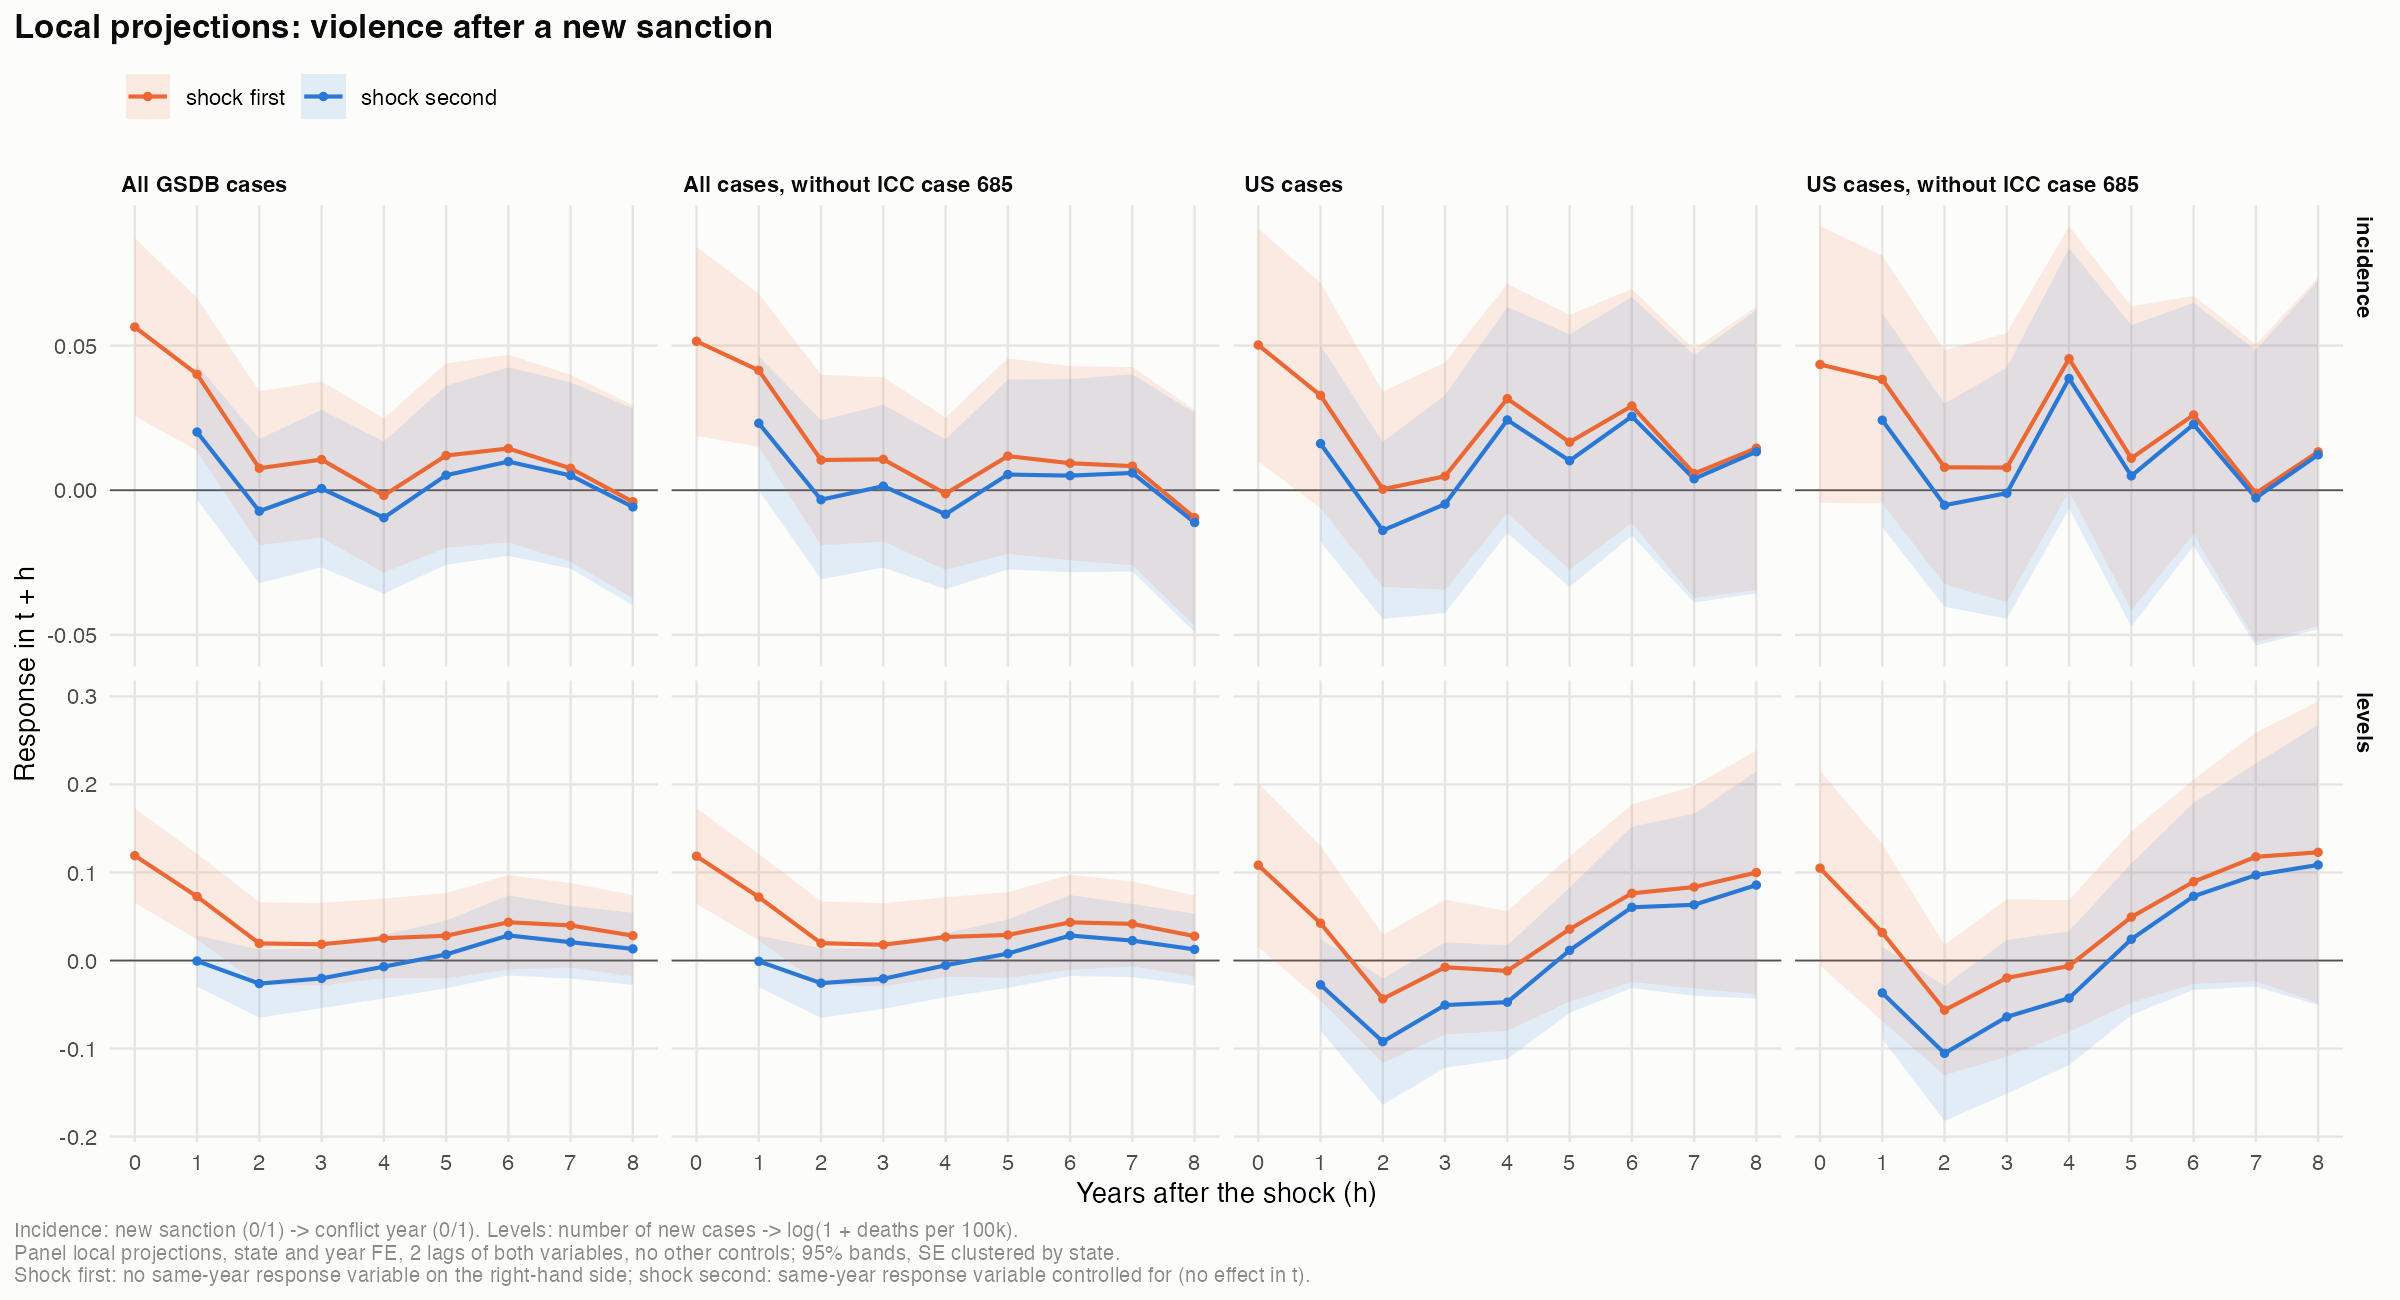
\includegraphics[width=0.8\textwidth]{fig18_lp_sanctions_to_violence.png}
\caption{Sanctions $\rightarrow$ violence by sanction measure (UCDP). The only interval that excludes zero at
$h=2$ is US without 685, levels, shock second ($-0.105$, 95\,\% CI $[-0.18,-0.03]$). With shock first:
$-0.056$, $[-0.13, 0.02]$.}
\label{fig:lp}
\end{figure}

Violence $\rightarrow$ sanctions: a conflict year raises the cumulative probability of a new sanction by $+0.21$ (all
cases) and $+0.09$ (US without 685) over 2--3 years, in both timings.

% -----------------------------------------------------------------------------
\section{Specification curves}
\label{sec:grid}

All combinations of the following choices were estimated (\texttt{specifications.R}, scripts 15--16):
\begin{itemize}[leftmargin=*]
\item violence source: UCDP, ACLED or GDELT;
\item sanction measure: eight versions;
\item levels or incidence;
\item sample: all states, states in conflict in $t-1$, or without Israel;
\item years: each source's own coverage, or the common window;
\item fixed effects: state or region, each with year;
\item timing and controls.
\end{itemize}
This gives 3{,}360 specifications. Levels are in SD units of each source, so the sources are comparable.

\textbf{How to read the curves.} Each column is one specification. The top panel shows its estimate and 95\,\%
interval, sorted from most negative to most positive. Below it, each row is one option of one choice: a tick in a
column means that specification uses the option. Tick colours repeat the significance of the estimate. Where an
option's ticks bunch at the left, that option produces the most negative estimates; ticks spread evenly mean the
option does not move the answer. Figure~\ref{fig:specshares} summarises the same information as shares.

\begin{figure}[H]
\centering
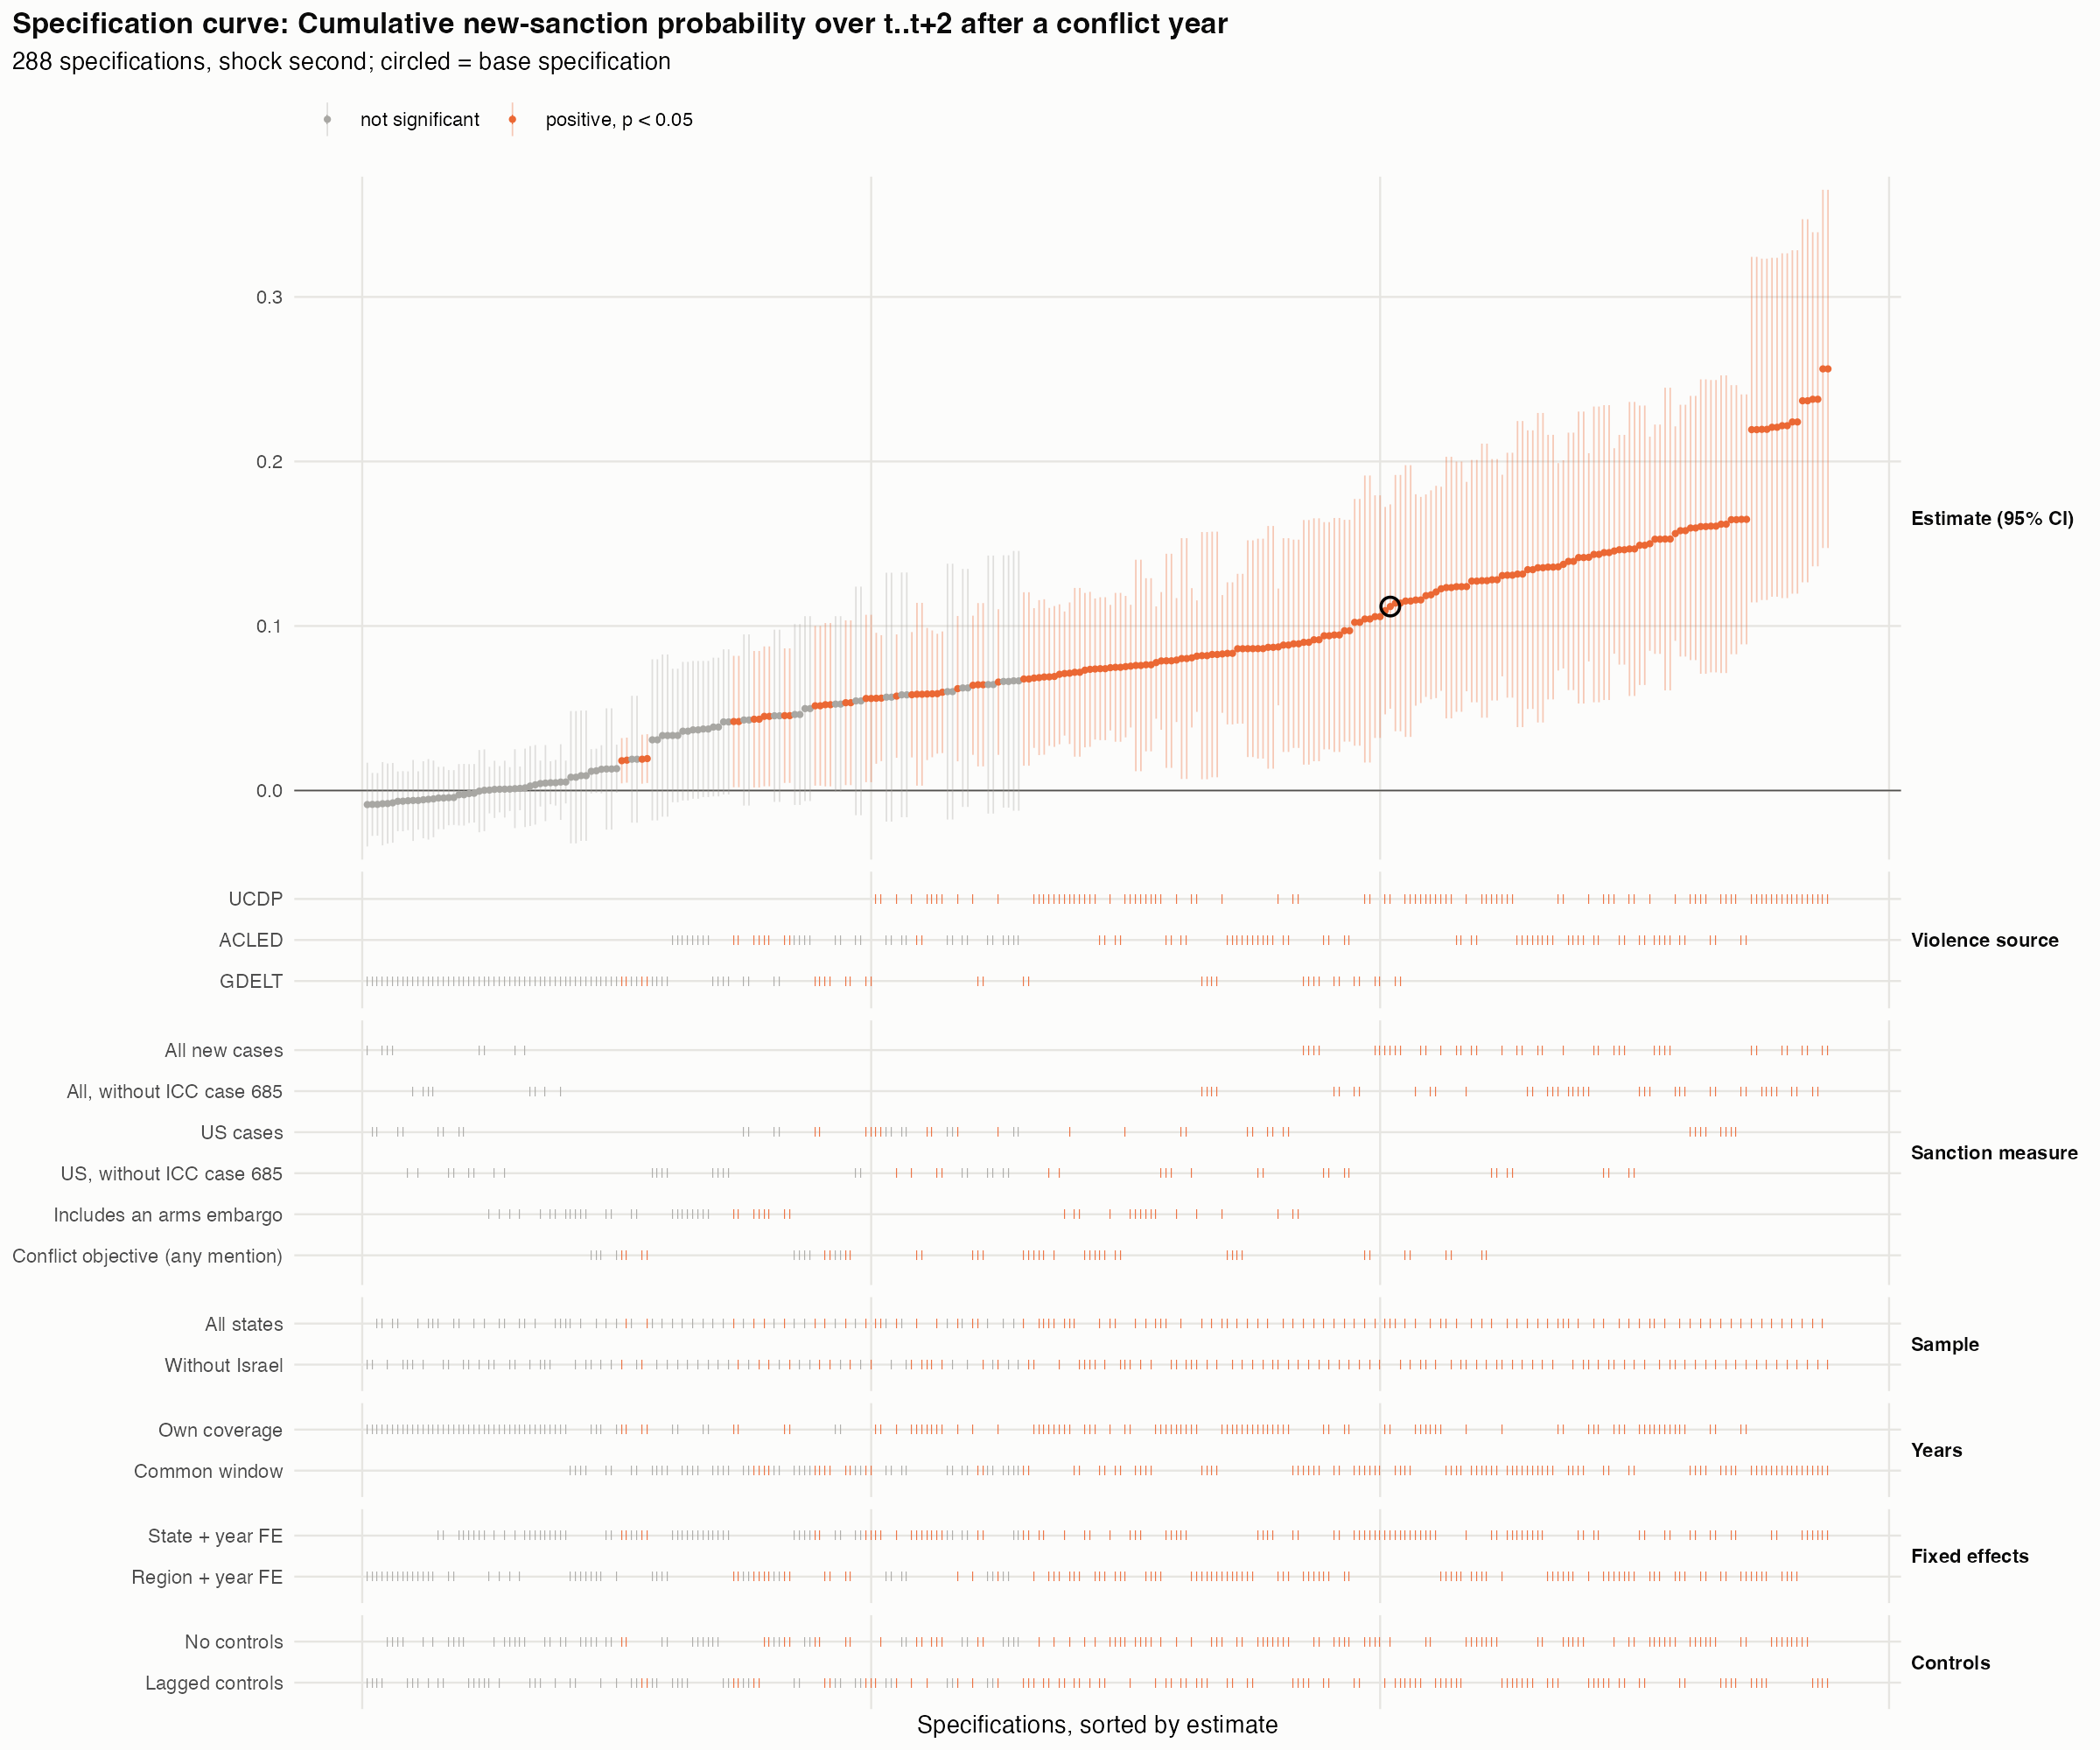
\includegraphics[width=0.72\textwidth]{fig23_spec_curve_sanctions_cum2.png}
\caption{Violence $\rightarrow$ sanctions: cumulative new-sanction probability over $t..t+2$ after a conflict year,
288 specifications. Median $+0.074$; significant in all UCDP specifications, 69\,\% of ACLED and 33\,\% of GDELT
(the grey block on the left is mostly GDELT).}
\label{fig:specv2s}
\end{figure}

\begin{figure}[H]
\centering
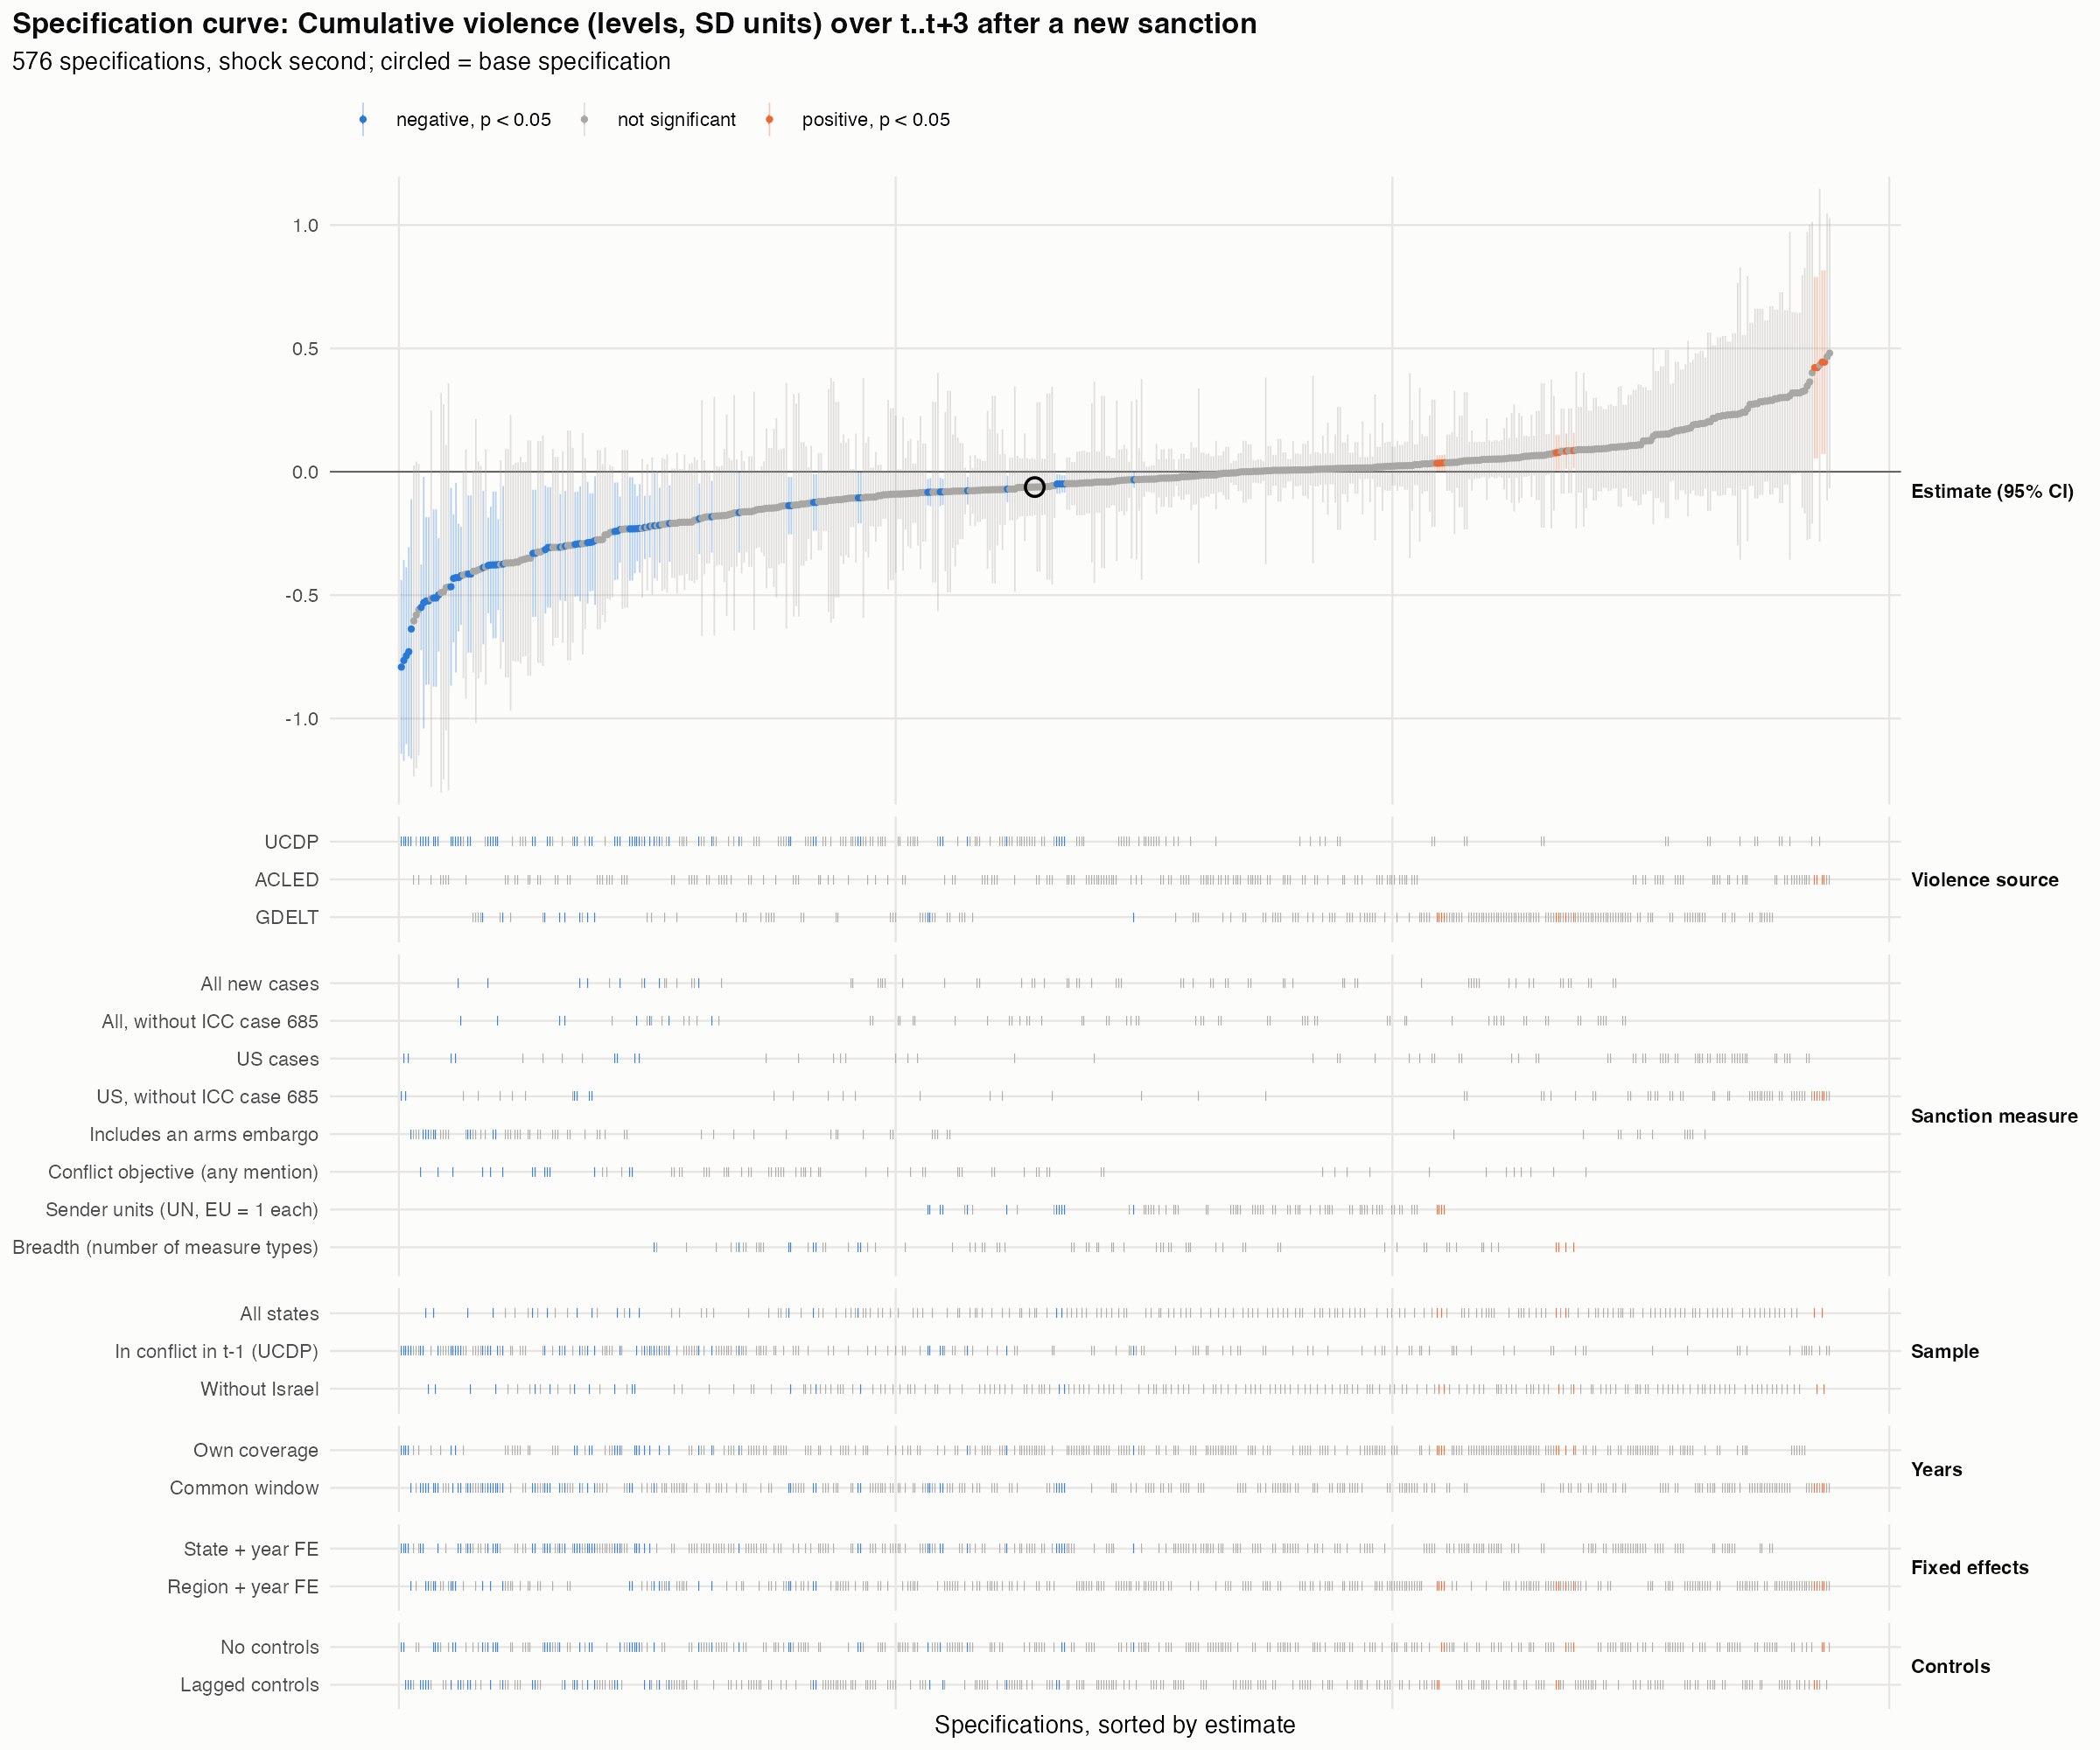
\includegraphics[width=0.72\textwidth]{fig23_spec_curve_deaths_cum3.png}
\caption{Sanctions $\rightarrow$ violence: cumulative deaths over $t..t+3$ (SD units), 576 specifications. Median
$-0.038$; 13\,\% significantly negative, 2\,\% significantly positive.}
\label{fig:specdeaths}
\end{figure}

\begin{figure}[H]
\centering
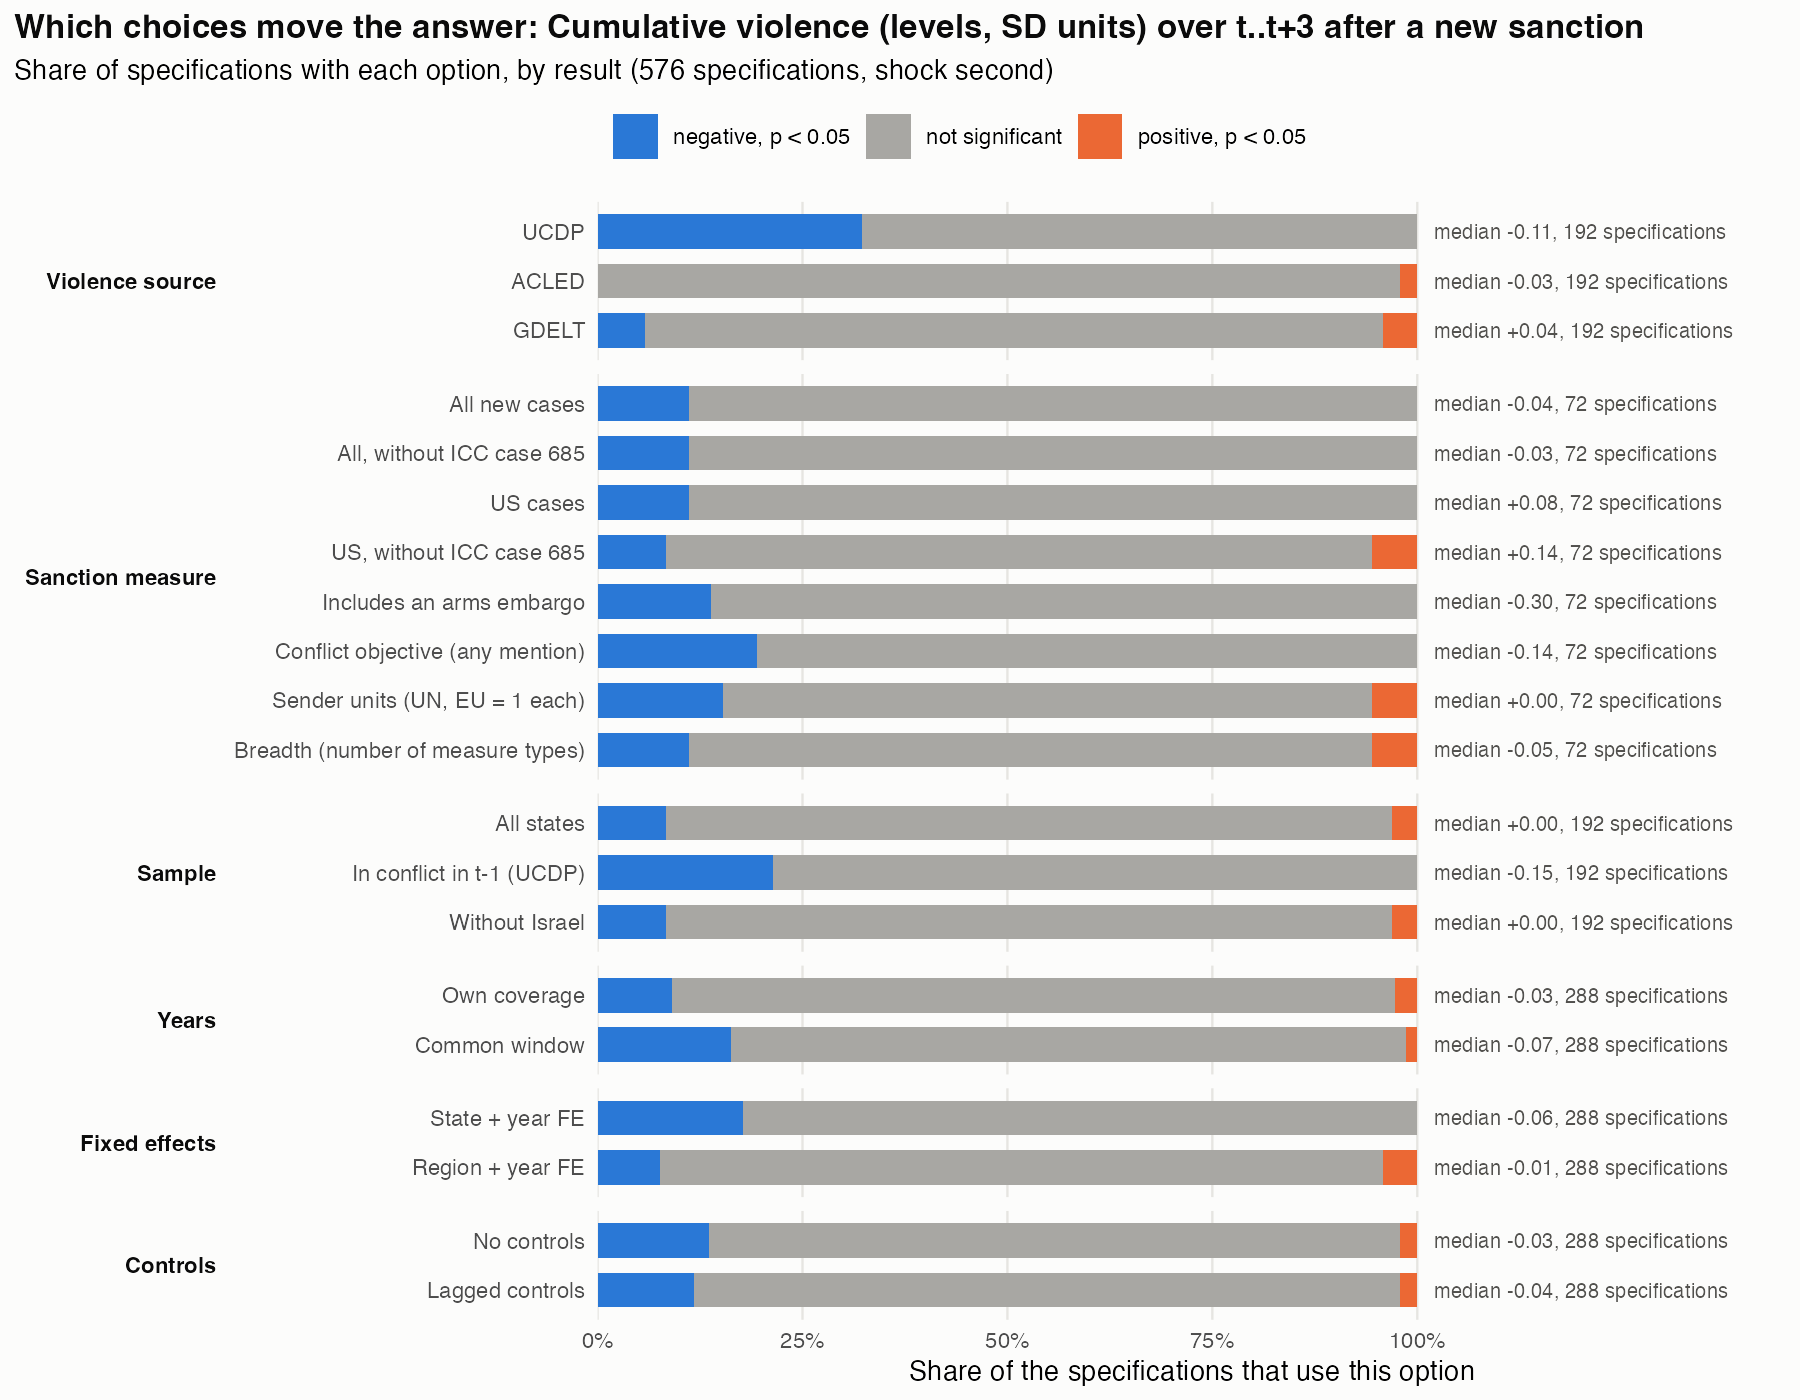
\includegraphics[width=0.68\textwidth]{fig23b_spec_dimensions_deaths_cum3.png}
\caption{The curve of Figure~\ref{fig:specdeaths} by option: share of specifications with a significant negative,
insignificant, or significant positive estimate, and the median estimate.}
\label{fig:specshares}
\end{figure}

What the shares show:
\begin{itemize}[leftmargin=*]
\item \textbf{Source.} UCDP: 32\,\% significantly negative, median $-0.11$. ACLED: none. GDELT: median $+0.04$.
\item \textbf{Sanction measure.} Arms embargo and conflict objective have the most negative medians ($-0.30$, $-0.14$),
  but only 14\,\% and 19\,\% of their specifications are significant. The US measures have positive medians
  ($+0.08$; $+0.14$ without 685).
\item \textbf{Sample.} The in-conflict sample has median $-0.15$, with 21\,\% significant.
\item \textbf{Other choices.} Fixed effects, years and controls change little.
\end{itemize}
Conflict incidence at $h=2$ is never significant (432 specifications).

% -----------------------------------------------------------------------------
\section{The US effect: where it comes from}
\label{sec:us}

\begin{figure}[H]
\centering
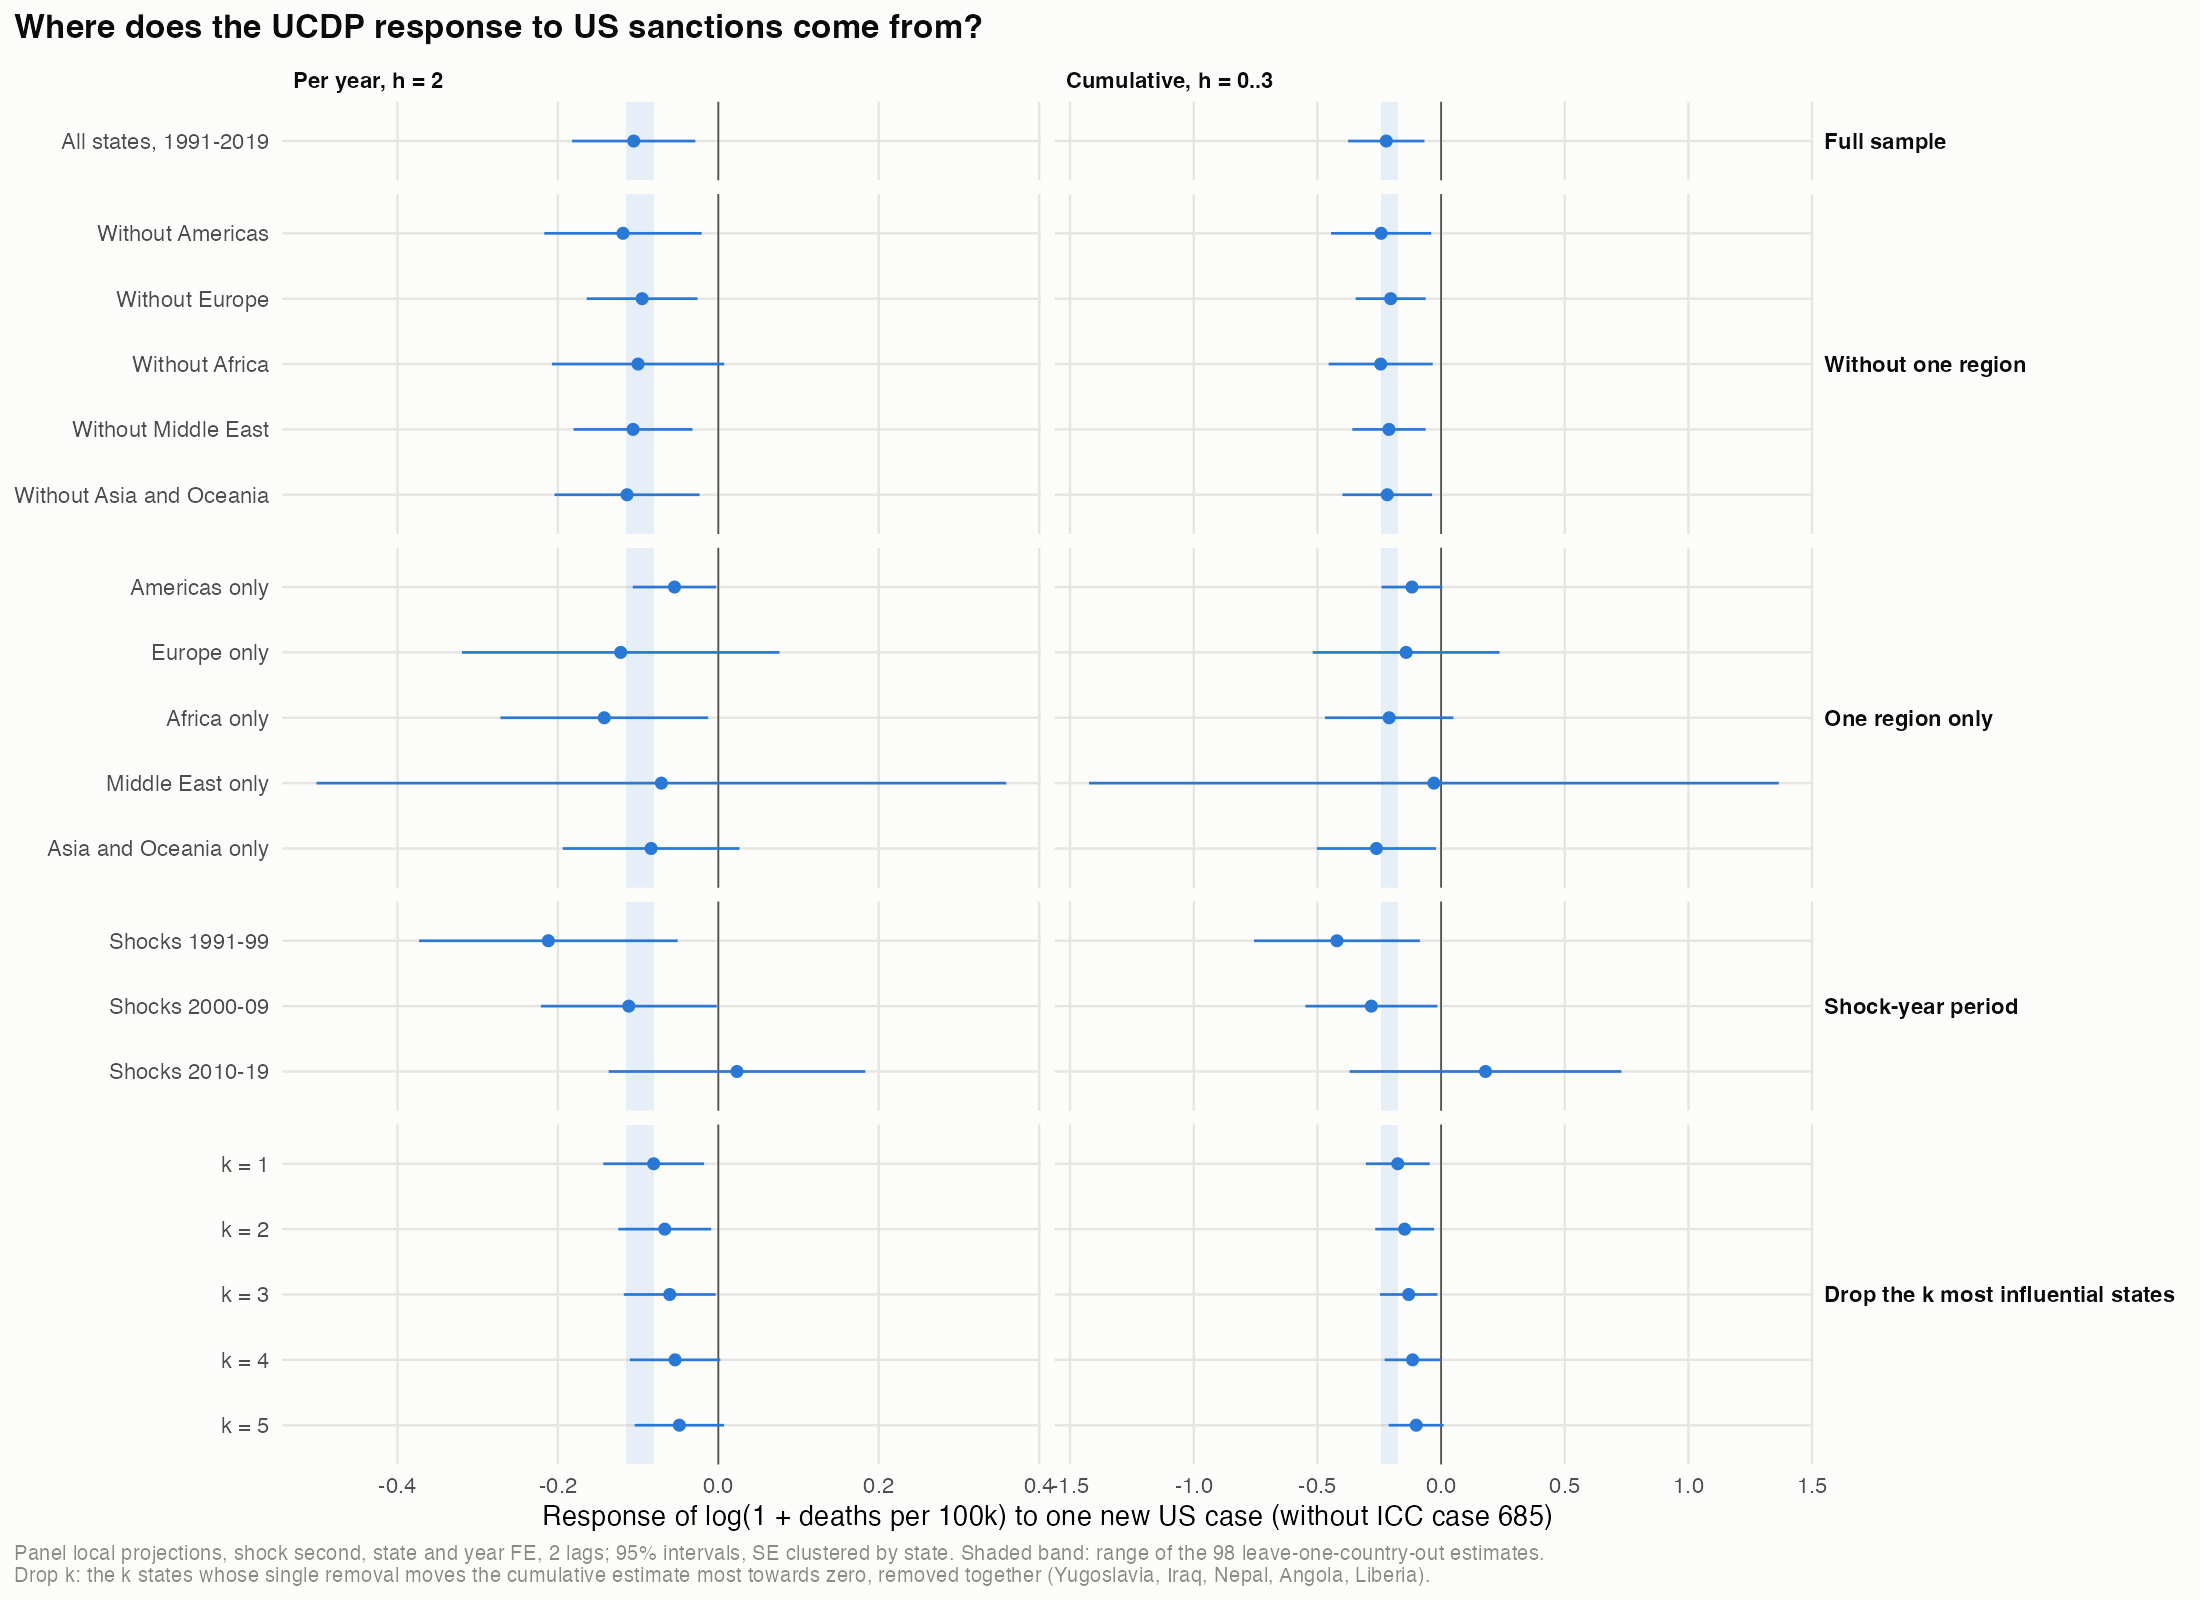
\includegraphics[width=0.62\textwidth]{fig24_lp_us_effect_location.png}
\caption{US effect (without 685, levels, shock second) at $h=2$ and cumulative $h=0..3$ in sub-samples.}
\label{fig:location}
\end{figure}

\begin{itemize}[leftmargin=*]
\item \textbf{Not one region.} Leaving out any region gives $-0.095$ to $-0.119$.
\item \textbf{A 1990s--2000s pattern.} By decade of the shock: $-0.21$\sig{**} (1991--99), $-0.11$\sig{**} (2000--09),
  $+0.02$ (2010--19).
\item \textbf{A handful of wars.} Dropping any single country keeps $p<0.05$, but dropping Yugoslavia, Iraq, Nepal,
  Angola and Liberia together halves the effect ($-0.049$\sig{*}).
\item \textbf{Objective.} The decline follows both conflict-objective cases ($-0.145$\sig{*}) and other cases
  ($-0.090$\sig{**}); the difference is not significant.
\end{itemize}

% -----------------------------------------------------------------------------
\section{Arms embargoes in ongoing wars}
\label{sec:arms}

Sample: state-years in conflict in $t-1$ (1{,}130 state-years, 104 states, 1991--2019). A new arms embargo $A_{it}$
and all other new cases $O_{it}$ enter separately (\texttt{14\_conflict\_sample\_lp.R}):
\begin{equation}
  y_{i,t+h} = \beta_h A_{it} + \gamma_h O_{it}
  + \sum_{k=1}^{2}\big(\phi_{hk} A_{i,t-k} + \psi_{hk} O_{i,t-k} + \rho_{hk}' \mathbf{y}_{i,t-k}\big)
  + \rho_{h0}' \mathbf{y}_{it} + \mu_{i} \text{ (or } \mu_{r(i)}) + \tau_t + \varepsilon_{i,t+h},
\end{equation}
with $\mathbf{y} = (\text{incidence}, \log \text{deaths})$.

\begin{figure}[H]
\centering
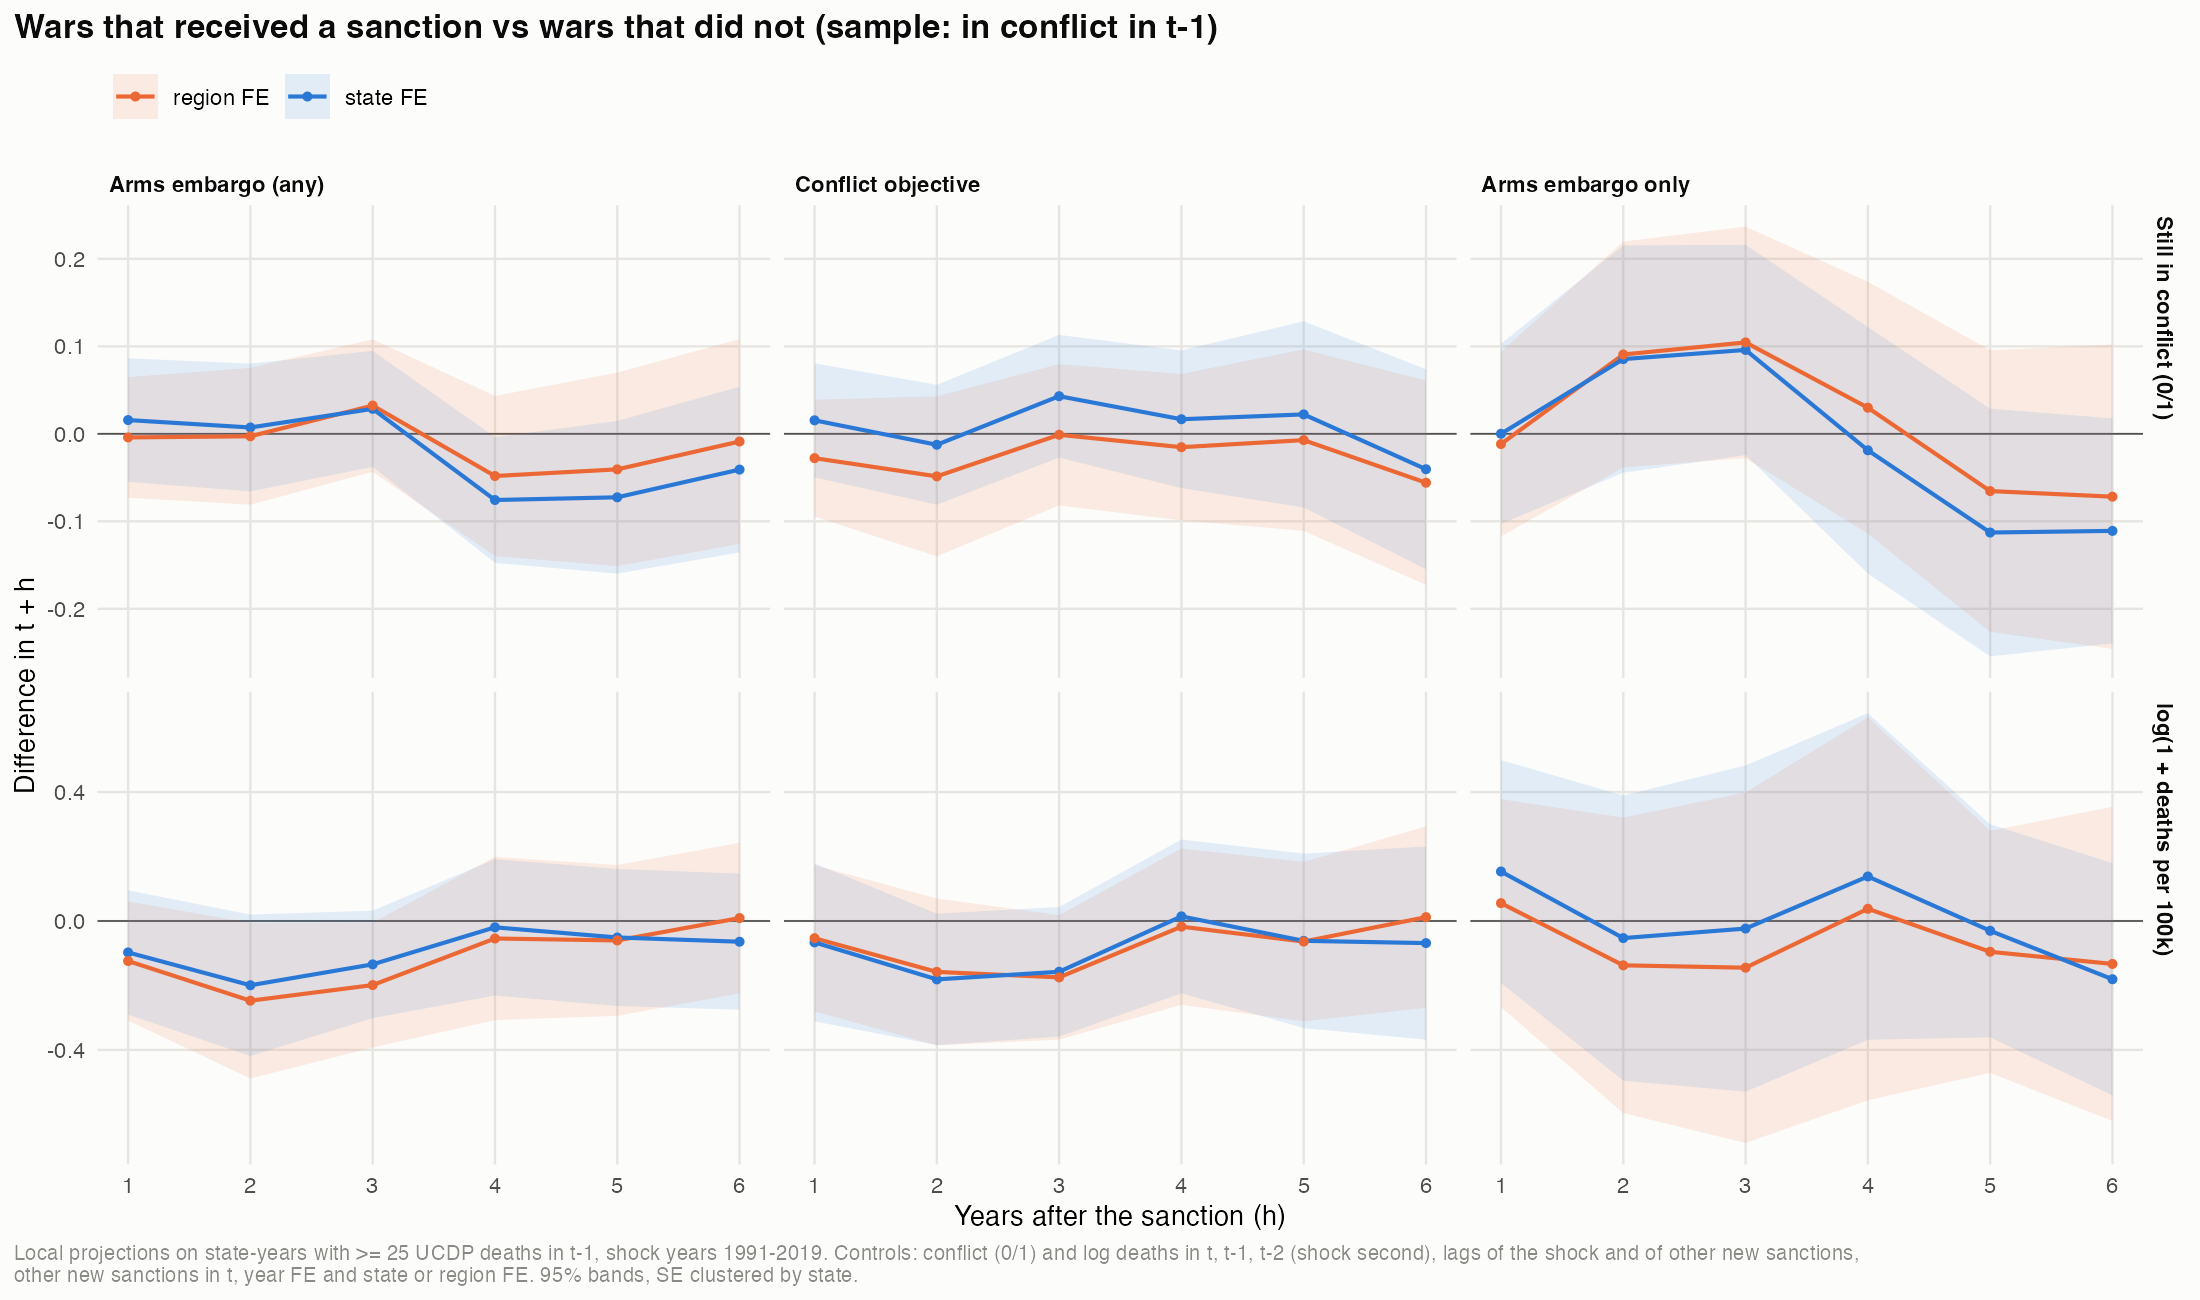
\includegraphics[width=0.72\textwidth]{fig22_conflict_sample_lp.png}
\caption{Wars with a new sanction vs.\ wars without, by type. Includes an arms embargo: deaths $-0.25$\sig{**} (region
FE) / $-0.20$\sig{*} (state FE) at $h=2$; cumulative $h=3$ $-0.57$\sig{**} / $-0.45$\sig{**}. Whether the war continues:
no change. Arms embargo only: nothing (28 events).}
\label{fig:arms}
\end{figure}

% -----------------------------------------------------------------------------
\section{ACLED and Africa}
\label{sec:acled}

\begin{figure}[H]
\centering
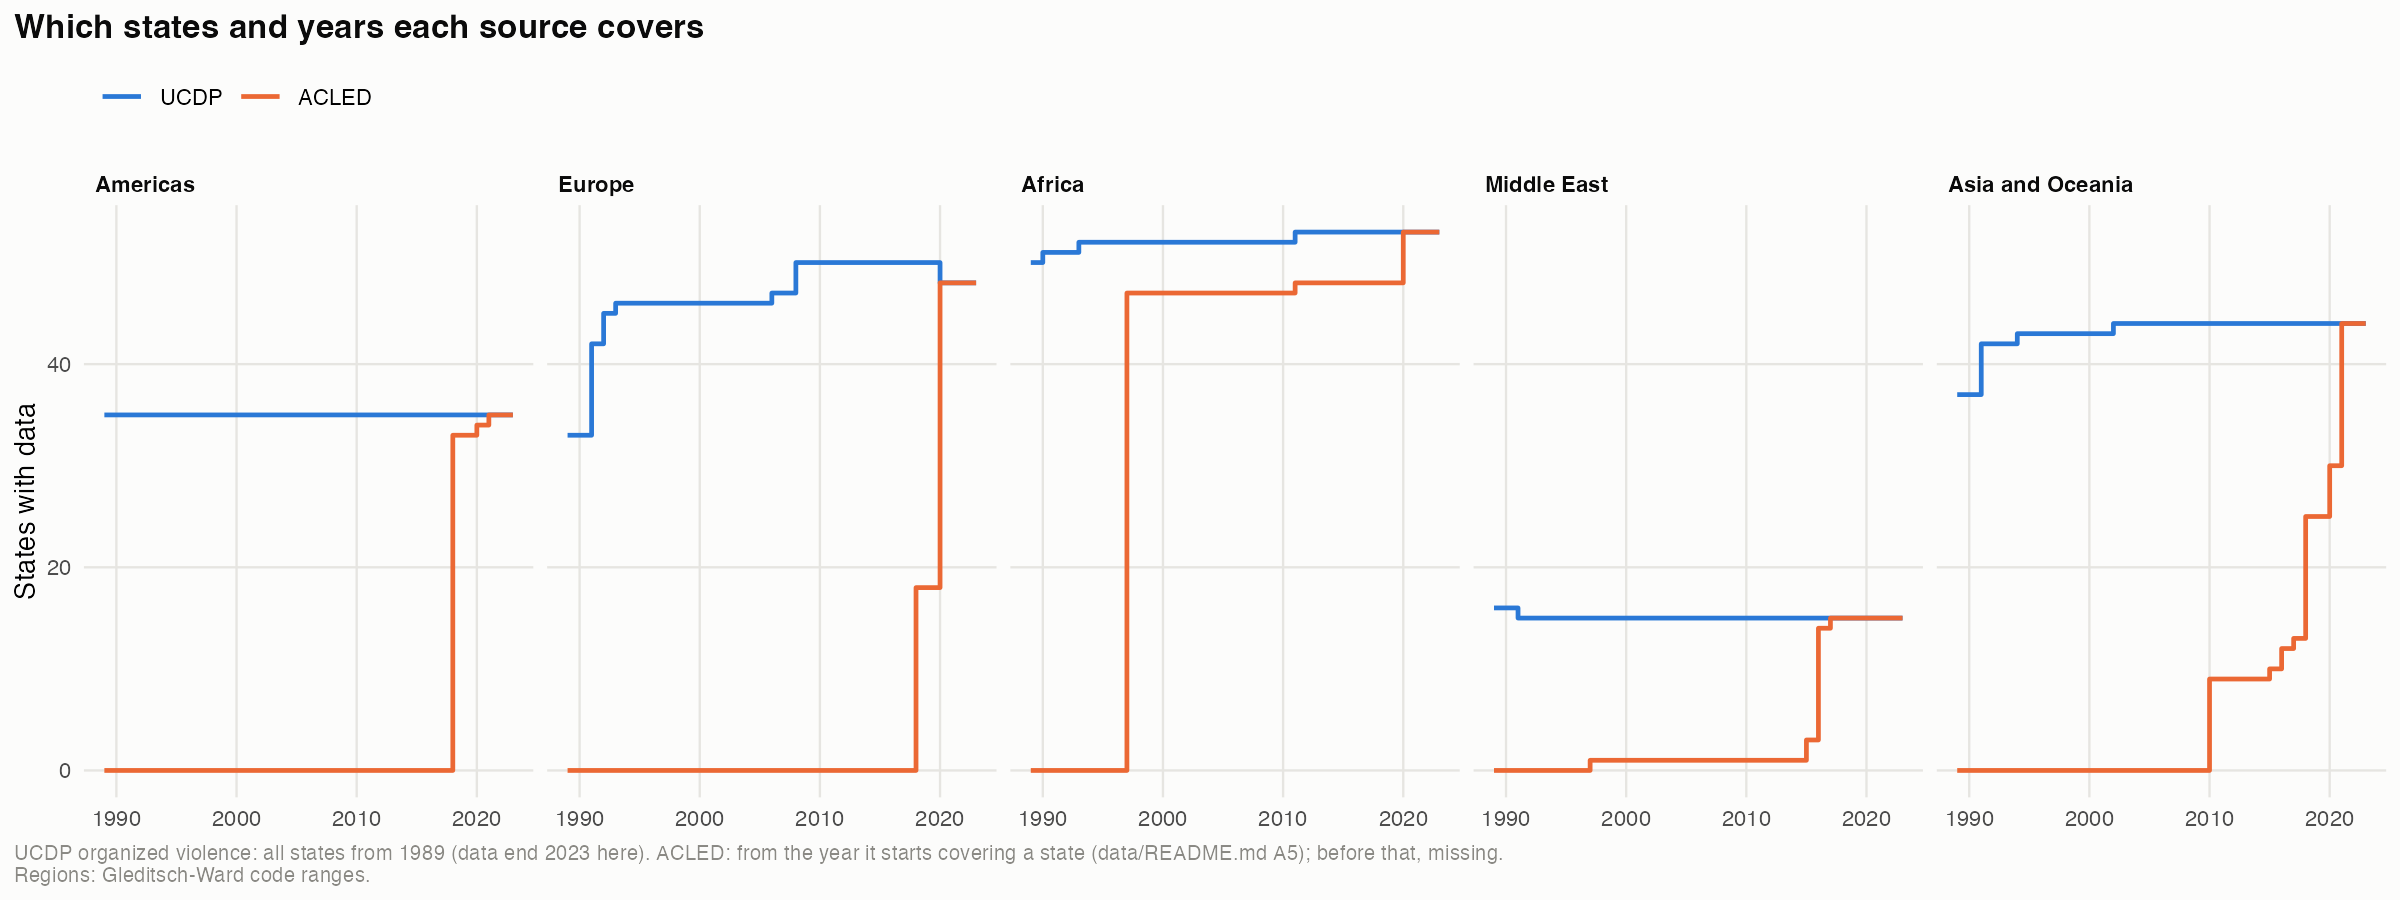
\includegraphics[width=0.85\textwidth]{fig26_sources_coverage.png}
\caption{States covered by UCDP and ACLED over time, by region.}
\label{fig:coverage}
\end{figure}

\textbf{ACLED is mainly an Africa sample} (Figure~\ref{fig:coverage}).
\begin{itemize}[leftmargin=*]
\item \textbf{Coverage.} Africa is covered from 1997. Asia comes in gradually from 2010, the Middle East from 2016,
  and the Americas and Europe only from 2018--2020.
\item \textbf{US events.} Of 142 US sanction events in the ACLED sample, 116 are in Africa and 119 are from 2010--2023.
  UCDP has 244, 63 of them before 1997.
\item \textbf{Same state-years, same answer.} ACLED finds no decline after US sanctions, and neither does UCDP on the
  same state-years (cumulative $h=2$: UCDP $-0.03$, ACLED $+0.03$).
\item \textbf{Sample, not measurement.} The two sources agree on log deaths (correlation 0.85--0.99 by region,
  Americas 0.39). The difference from the full-sample UCDP result comes from the sample.
\end{itemize}

\textbf{Africa: many sanctions, few in the ACLED estimates.} In absolute terms Africa is not under-sanctioned
(Table~\ref{tab:regions}). It has a third of all new-case state-years, more than half of the UN cases and almost
half of the arms embargoes. Relative to its many conflict years, however, it does not receive more than other
regions. In the Africa-only LP on the ACLED window (script 18) only 28 UN events and 40 arms embargoes remain. The
only intervals that exclude zero are single-year declines at $h=1$:
\begin{itemize}[leftmargin=*]
\item after UN sanctions: $-0.29$\sig{***} (UCDP), $-0.22$\sig{***} (ACLED);
\item after arms embargoes: $-0.19$\sig{***} (UCDP), $-0.15$\sig{**} (ACLED).
\end{itemize}
This is suggestive at most.

\begin{table}[H]
\centering\small
\caption{New-case state-years by region, 1991--2019 (without case 685)}
\label{tab:regions}
\setlength{\tabcolsep}{4pt}
\begin{tabular}{@{}lrrrrrrrr@{}}
\toprule
 & & State- & Conflict & Any new & & & Arms & per 100 \\
Region & States & years & years & case & US & UN & embargo & st.-years \\
\midrule
Africa      & 52 & 1{,}506 & 477 & 174 & 78 & 36 & 65 & 11.6 \\
Middle East & 15 &    435 & 169 &  51 & 22 & 15 & 18 & 11.7 \\
Europe      & 51 & 1{,}377 &  79 & 131 & 26 &  4 & 18 &  9.5 \\
Asia        & 44 & 1{,}262 & 264 & 100 & 50 &  8 & 32 &  7.9 \\
Americas    & 35 & 1{,}015 & 137 &  63 & 49 &  2 &  8 &  6.2 \\
\midrule
Total       & 197 & 5{,}595 & 1{,}126 & 519 & 225 & 65 & 141 & 9.3 \\
\bottomrule
\end{tabular}
\end{table}

% -----------------------------------------------------------------------------
\section{Trade and arms exposure (first look)}
\label{sec:exposure}

\textbf{Data.} Three new sources: WDI (trade and FDI over GDP, SIPRI arms totals), IMF IMTS bilateral goods trade
(217 reporters, 1980--2025), and SIPRI arms transfers (bilateral TIV and the transfer register, 1950--2025).

\textbf{Exposure.} $Z_{it}$ is the target's exposure to the sender: the mean over $t-3..t-1$, standardised. Three
measures: trade with the sender over GDP, the sender's share of trade, and the sender's share of arms imports. Each
is built for the US, for EU members of the year, and for the actual senders of each case. The LP adds an
interaction:
\begin{equation}
  y_{i,t+h} = b_h x_{it} + c_h\, x_{it} Z_{it} + d_h Z_{it} + \text{history} + c'_h y_{it} + \mu_i + \tau_t + \varepsilon_{i,t+h}.
\end{equation}

\textbf{Trade.} $c_h \approx 0$ in UCDP and ACLED for US, EU and all-case senders, also with alternative coding of
missing trade, by terciles, and in the in-conflict sample. GDELT, if anything, shows more reported violence.

\textbf{Arms.} Split into no / some / high arms dependence on the sender (Figure~\ref{fig:exposure}), 27 cells in all
(3 senders $\times$ 3 groups $\times$ 3 sources). No pattern is consistent across sources. One cell is negative in
both UCDP and ACLED: EU sanctions on targets with high EU arms dependence ($-0.31$\sig{**} with 17 events;
$-0.45$\sig{*} with 8). With so few events and so many cells this is not a result. The arms channel needs a different
design, such as arms flows as the outcome.

\begin{figure}[H]
\centering
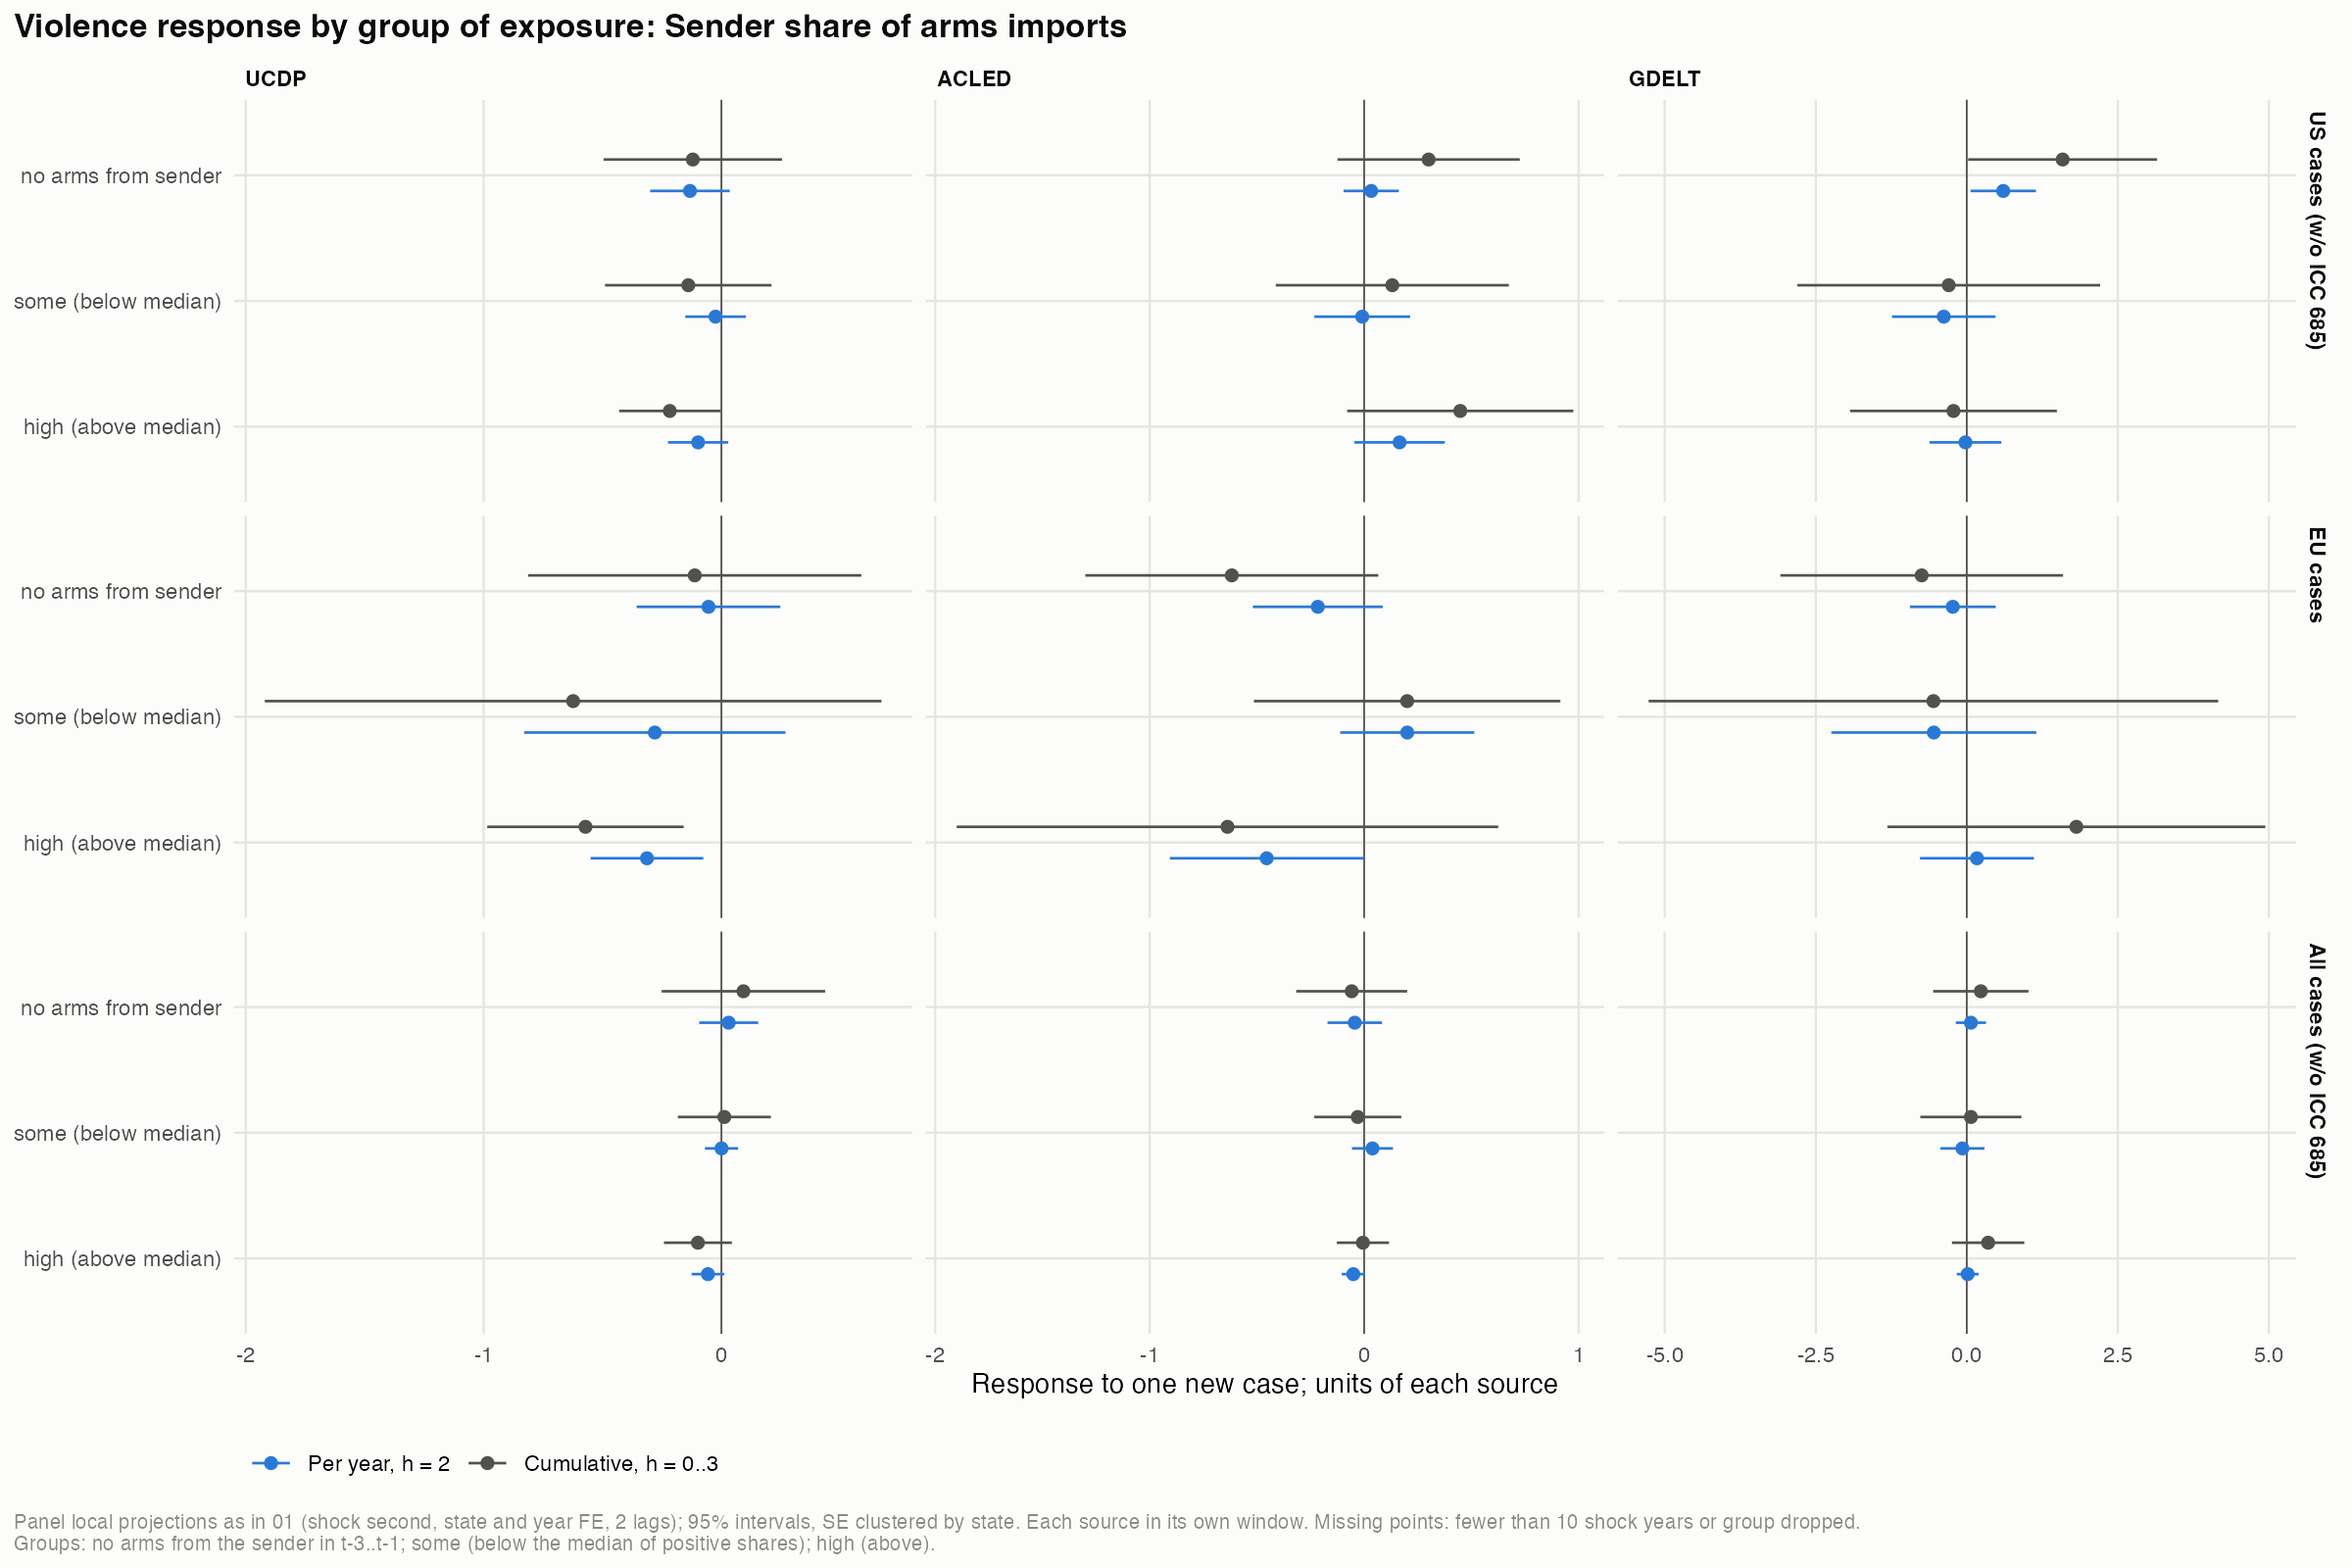
\includegraphics[width=0.68\textwidth]{fig_e3_groups_arms.png}
\caption{Response by the target's arms dependence on the sender (no / some / high share of arms imports).}
\label{fig:exposure}
\end{figure}

% =============================================================================
\parttitle{Part B --- Towards causal estimates}
% =============================================================================

\section{What local projections can and cannot do}
\label{sec:identification}

LP estimates each horizon directly instead of iterating a one-step VAR. In population both target the same impulse
response \citep{plagborg2021}; LP has less bias and more variance \citep{li2024}. Neither is an identification
strategy. Both read $\beta_h$ causally only under selection on observables:
\begin{equation}
  \big\{y_{i,t+h}(1),\, y_{i,t+h}(0)\big\} \;\perp\; D_{it} \;\big|\; X_{it},\ \mu_i,\ \tau_t ,
  \label{eq:cia}
\end{equation}
i.e.\ given a state's recent violence and sanction history, the timing of a sanction is as good as random. This
fails if senders act on information outside $X_{it}$, if sanctions come bundled with other interventions, or if the
annual ordering of sanction and violence is wrong.

The recent literature offers three ways forward:
\begin{enumerate}[leftmargin=*]
\item \textbf{Model the policy decision and reweight} \citep{angrist2018,jordataylor2016}. Double ML
  \citep{chernozhukov2018} is the machine-learning version.
\item \textbf{LP-DiD} with clean controls and pre-trends \citep{dube2025}: a parallel-trends counterpart that brackets
  the estimate.
\item \textbf{LP-IV} with an instrument \citep{stock2018}. There is no credible candidate yet.
\end{enumerate}
Two further points from the literature:
\begin{itemize}[leftmargin=*]
\item A linear LP with an observed shock recovers a positively weighted average of heterogeneous effects
  \citep{kolesar2025}, so its sign is interpretable.
\item Panel LP with fixed effects needs a bias correction \citep{herbst2024,mei2026}.
\end{itemize}
Recent related applied work: \citet{farzanegan2026}.

% -----------------------------------------------------------------------------
\section{The Jordà--Taylor approach: doubly robust local projections}
\label{sec:jt}

Treatment: $D_{it} = \mathds{1}[\text{new US case in } t]$, without case 685. Script:
\texttt{doubly\_robust/scripts/\allowbreak 01\_dr\_lp.R}.

\textit{Step 1, propensity score = sanction reaction function:}
\begin{gather}
  p(X_{it}) = \Pr(D_{it}=1 \mid X_{it}) = \Lambda\big(\delta' X_{it} + \rho_{r(i)} + \pi_{\text{5-yr}(t)}\big), \\
  X_{it} = \big(y_{it},\, y_{i,t-1},\, y_{i,t-2},\, D_{i,t-1},\, D_{i,t-2}\big). \notag
\end{gather}

\textit{Step 2, common support:} $0<p(X)<1$, checked by the min/max rule \citep{crump2009}
\[
  \Big[\max\big(\min_{D=1}\hat p,\ \min_{D=0}\hat p\big),\ \ \min\big(\max_{D=1}\hat p,\ \max_{D=0}\hat p\big)\Big].
\]

\textit{Step 3, weighted LP.} The weights are
$w^{\text{ATE}}_{it} = \frac{D_{it}}{\hat p_{it}} + \frac{1-D_{it}}{1-\hat p_{it}}$ and
$w^{\text{ATT}}_{it} = D_{it} + (1-D_{it})\frac{\hat p_{it}}{1-\hat p_{it}}$.
\begin{itemize}[leftmargin=*]
\item IPW regresses $y_{i,t+h}$ on $D_{it}$ and the fixed effects, with these weights.
\item IPWRA estimates \eqref{eq:lp} with the same weights. It is doubly robust \citep{wooldridge2007}: consistent if
  either the propensity model or the outcome regression is correct.
\end{itemize}
The AIPW form in \citet{jordataylor2016} is
\begin{equation}
\begin{split}
  \hat\theta_h = \frac{1}{N}\sum_{i,t}\Big[\, & \hat m_1(X_{it}) - \hat m_0(X_{it}) \\
  & + \frac{D_{it}\big(y_{i,t+h}-\hat m_1(X_{it})\big)}{\hat p_{it}}
    - \frac{(1-D_{it})\big(y_{i,t+h}-\hat m_0(X_{it})\big)}{1-\hat p_{it}}\Big],
\end{split}
\end{equation}
where $\hat m_d(X_{it})$ is the predicted outcome $y_{i,t+h}$ under treatment status $d$, from the outcome regression.

\begin{figure}[H]
\centering
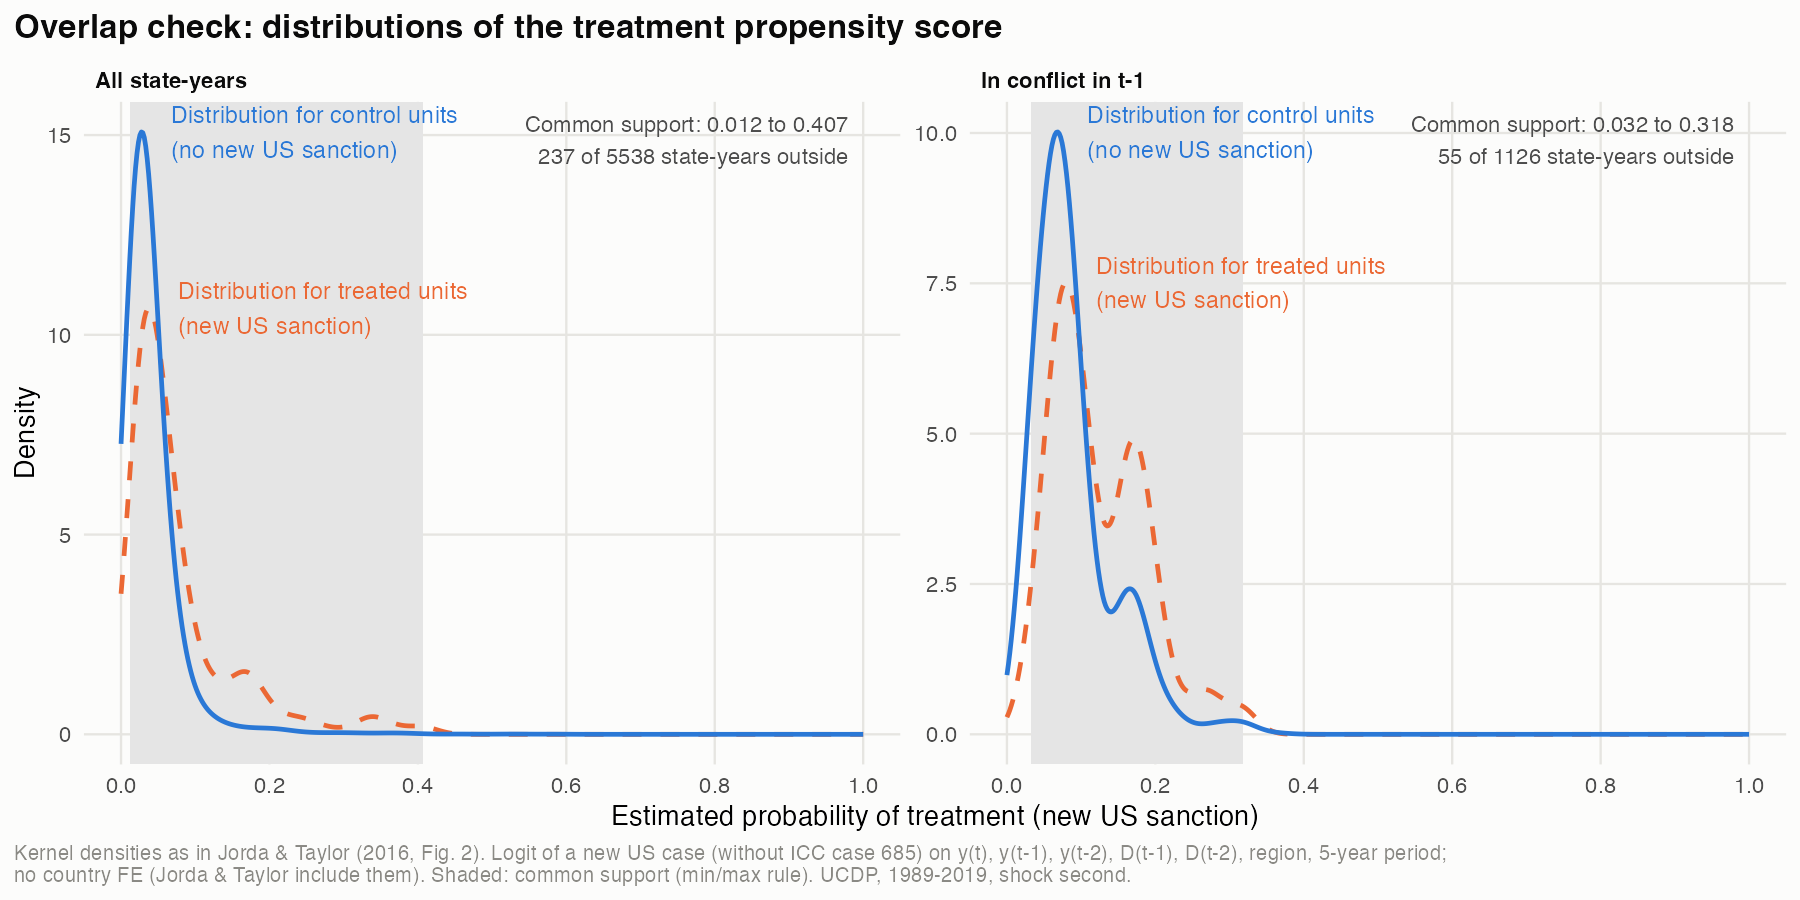
\includegraphics[width=0.8\textwidth]{dr4_common_support.png}
\caption{Overlap check, drawn as in \citet[Fig.~2]{jordataylor2016}. Shaded: common support, the intersection of
the two groups' ranges of $\hat p$. Sanctioned state-years range over 0.012--0.407 (in conflict: 0.032--0.318); the
controls range more widely (0.007--0.583; 0.017--0.362). The intersection therefore equals the sanctioned range: every
sanctioned state-year is inside it, and only controls lie outside (232 below, 5 above; in conflict 50 below, 5 above).
The curves are smoothed and spill slightly beyond the actual ranges. The two densities nearly coincide (AUC 0.72 /
0.68, against 0.86 in Jordà--Taylor): US sanctions are hard to predict from the observed history.}
\label{fig:cs}
\end{figure}

\begin{figure}[H]
\centering
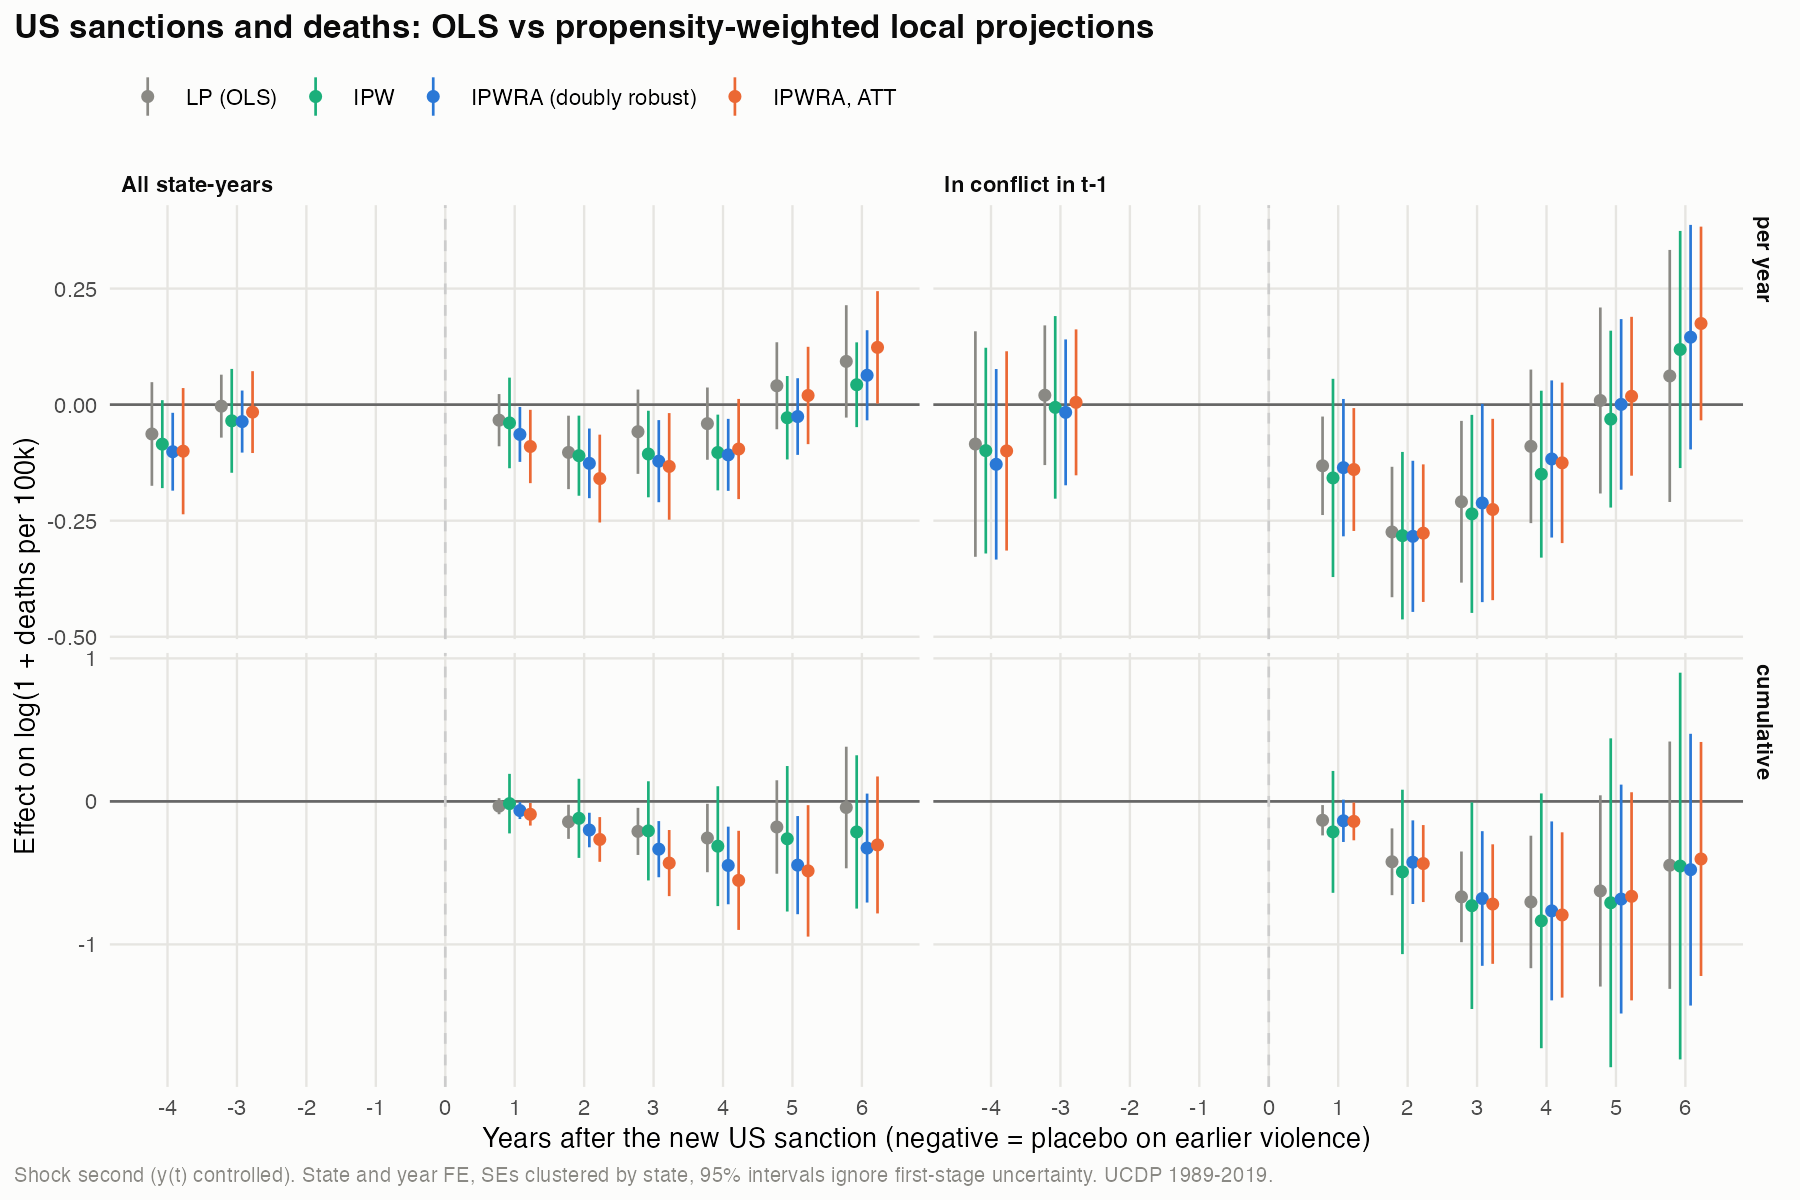
\includegraphics[width=0.72\textwidth]{dr3_lp_paths.png}
\caption{OLS vs.\ propensity-weighted LP by year; negative years are placebos (violence before the sanction).}
\label{fig:dr}
\end{figure}

\begin{table}[H]
\centering\small
\caption{US sanctions $\rightarrow$ log deaths: OLS vs.\ propensity-weighted LP (shock second), first implementation}
\label{tab:dr}
\begin{tabular}{@{}lcccc@{}}
\toprule
 & OLS & IPW & IPWRA (DR) & IPWRA, ATT \\
\midrule
All state-years, $h=2$            & $-0.103$\sig{**}  & $-0.110$\sig{**}  & $-0.127$\sig{***} & $-0.159$\sig{***} \\
All state-years, cum.\ $h=0..3$   & $-0.210$\sig{**}  & $-0.206$          & $-0.334$\sig{***} & $-0.431$\sig{***} \\
In conflict in $t-1$, $h=2$       & $-0.274$\sig{***} & $-0.282$\sig{***} & $-0.284$\sig{***} & $-0.277$\sig{***} \\
Placebo: $y_{t-3}$, all           & $-0.003$          & $-0.035$          & $-0.036$          & $-0.016$ \\
\bottomrule
\end{tabular}
\end{table}

\textbf{Status.} This is a first run, and no conclusions should be drawn from it yet. Open items:
\begin{itemize}[leftmargin=*]
\item The propensity model is minimal: two lags, no country fixed effects.
\item Standard errors treat $\hat p$ as known.
\item Two of 32 placebo estimates exclude zero, both for $y_{t-4}$ with IPWRA-ATE in all state-years (about what chance gives).
\item The design choices (binary treatment, covariates, trimming at 0.01, ATE vs.\ ATT) are defaults.
\end{itemize}
The low AUC cuts both ways. The comparison is well supported on observables, but most of what drives US sanctions
is not in the data.

% -----------------------------------------------------------------------------
\section{The pattern to explain, and next steps}
\label{sec:next}

Sanctions arrive in violent state-years, and in UCDP violence then falls faster than in equally violent
state-years without sanctions. Linear mean reversion is netted out by the controls in \eqref{eq:lp}. The open
question is why the two coincide:

\begin{table}[H]
\centering\small
\caption{Explanations for the decline after sanctions and how to tell them apart}
\label{tab:explanations}
\begin{tabularx}{\textwidth}{@{}p{3.4cm}XX@{}}
\toprule
Explanation & Prediction & Test \\
\midrule
Sanctions work & larger decline where sanctions bite; a visible channel & arms embargo $\rightarrow$ arms imports (SIPRI) $\rightarrow$ deaths \\
Non-linear reversion, war phase & unsanctioned peaks fall just as fast & matched peaks, war age, episode phase (UCDP/PRIO episode dates) \\
Bundling & decline comes with peacekeeping, mediation, intervention & peacekeeping and peace-agreement data \\
Sender foresight & sanctions timed to an expected decline & monthly timing, case reading \\
\bottomrule
\end{tabularx}
\end{table}

\paragraph{Next steps.}
\begin{enumerate}[leftmargin=*]
\item \textbf{Arms channel, first link:} do arms imports (SIPRI TIV) fall after arms embargoes and other sanctions?
  Only if they do is a mediation analysis through arms trade worth doing. Mediation needs sequential ignorability, so
  it would be mechanism evidence, not a decomposition.
\item \textbf{Trade exposure} and \textbf{violence $\rightarrow$ sanctions}: develop further into reportable results.
\item \textbf{Event-time picture:} violence $t-5..t+5$ around US sanctions vs.\ propensity-weighted controls, to see
  whether sanctions come at the peak. Within wars, sanctioned years are only slightly more violent (standardised
  difference 0.12).
\item \textbf{Doubly robust LP:} a richer propensity model, a cluster bootstrap over both steps, leave-out-top-5,
  ACLED, and an arms-embargo treatment.
\end{enumerate}

\bibliographystyle{plainnat}
\bibliography{../../references,report_refs}

\end{document}
